\documentclass[a4paper]{article}
\usepackage{lmodern}
\usepackage{amssymb,amsmath}
\usepackage{ifxetex,ifluatex}
\usepackage{fixltx2e} % provides \textsubscript
\ifnum 0\ifxetex 1\fi\ifluatex 1\fi=0 % if pdftex
  \usepackage[T1]{fontenc}
  \usepackage[utf8]{inputenc}
\else % if luatex or xelatex
  \ifxetex
    \usepackage{mathspec}
  \else
    \usepackage{fontspec}
  \fi
  \defaultfontfeatures{Ligatures=TeX,Scale=MatchLowercase}
\fi
% use upquote if available, for straight quotes in verbatim environments
\IfFileExists{upquote.sty}{\usepackage{upquote}}{}
% use microtype if available
\IfFileExists{microtype.sty}{%
\usepackage{microtype}
\UseMicrotypeSet[protrusion]{basicmath} % disable protrusion for tt fonts
}{}
\usepackage[margin=1in]{geometry}
\usepackage{hyperref}
\hypersetup{unicode=true,
            pdftitle={Avaliação de um lote urbano pelo Método Involutivo Vertical},
            pdfauthor={Luiz Fernando Palin Droubi; Willian Zonato},
            pdfborder={0 0 0},
            breaklinks=true}
\urlstyle{same}  % don't use monospace font for urls
\usepackage{color}
\usepackage{fancyvrb}
\newcommand{\VerbBar}{|}
\newcommand{\VERB}{\Verb[commandchars=\\\{\}]}
\DefineVerbatimEnvironment{Highlighting}{Verbatim}{commandchars=\\\{\}}
% Add ',fontsize=\small' for more characters per line
\usepackage{framed}
\definecolor{shadecolor}{RGB}{248,248,248}
\newenvironment{Shaded}{\begin{snugshade}}{\end{snugshade}}
\newcommand{\KeywordTok}[1]{\textcolor[rgb]{0.13,0.29,0.53}{\textbf{#1}}}
\newcommand{\DataTypeTok}[1]{\textcolor[rgb]{0.13,0.29,0.53}{#1}}
\newcommand{\DecValTok}[1]{\textcolor[rgb]{0.00,0.00,0.81}{#1}}
\newcommand{\BaseNTok}[1]{\textcolor[rgb]{0.00,0.00,0.81}{#1}}
\newcommand{\FloatTok}[1]{\textcolor[rgb]{0.00,0.00,0.81}{#1}}
\newcommand{\ConstantTok}[1]{\textcolor[rgb]{0.00,0.00,0.00}{#1}}
\newcommand{\CharTok}[1]{\textcolor[rgb]{0.31,0.60,0.02}{#1}}
\newcommand{\SpecialCharTok}[1]{\textcolor[rgb]{0.00,0.00,0.00}{#1}}
\newcommand{\StringTok}[1]{\textcolor[rgb]{0.31,0.60,0.02}{#1}}
\newcommand{\VerbatimStringTok}[1]{\textcolor[rgb]{0.31,0.60,0.02}{#1}}
\newcommand{\SpecialStringTok}[1]{\textcolor[rgb]{0.31,0.60,0.02}{#1}}
\newcommand{\ImportTok}[1]{#1}
\newcommand{\CommentTok}[1]{\textcolor[rgb]{0.56,0.35,0.01}{\textit{#1}}}
\newcommand{\DocumentationTok}[1]{\textcolor[rgb]{0.56,0.35,0.01}{\textbf{\textit{#1}}}}
\newcommand{\AnnotationTok}[1]{\textcolor[rgb]{0.56,0.35,0.01}{\textbf{\textit{#1}}}}
\newcommand{\CommentVarTok}[1]{\textcolor[rgb]{0.56,0.35,0.01}{\textbf{\textit{#1}}}}
\newcommand{\OtherTok}[1]{\textcolor[rgb]{0.56,0.35,0.01}{#1}}
\newcommand{\FunctionTok}[1]{\textcolor[rgb]{0.00,0.00,0.00}{#1}}
\newcommand{\VariableTok}[1]{\textcolor[rgb]{0.00,0.00,0.00}{#1}}
\newcommand{\ControlFlowTok}[1]{\textcolor[rgb]{0.13,0.29,0.53}{\textbf{#1}}}
\newcommand{\OperatorTok}[1]{\textcolor[rgb]{0.81,0.36,0.00}{\textbf{#1}}}
\newcommand{\BuiltInTok}[1]{#1}
\newcommand{\ExtensionTok}[1]{#1}
\newcommand{\PreprocessorTok}[1]{\textcolor[rgb]{0.56,0.35,0.01}{\textit{#1}}}
\newcommand{\AttributeTok}[1]{\textcolor[rgb]{0.77,0.63,0.00}{#1}}
\newcommand{\RegionMarkerTok}[1]{#1}
\newcommand{\InformationTok}[1]{\textcolor[rgb]{0.56,0.35,0.01}{\textbf{\textit{#1}}}}
\newcommand{\WarningTok}[1]{\textcolor[rgb]{0.56,0.35,0.01}{\textbf{\textit{#1}}}}
\newcommand{\AlertTok}[1]{\textcolor[rgb]{0.94,0.16,0.16}{#1}}
\newcommand{\ErrorTok}[1]{\textcolor[rgb]{0.64,0.00,0.00}{\textbf{#1}}}
\newcommand{\NormalTok}[1]{#1}
\usepackage{longtable,booktabs}
\usepackage{graphicx,grffile}
\makeatletter
\def\maxwidth{\ifdim\Gin@nat@width>\linewidth\linewidth\else\Gin@nat@width\fi}
\def\maxheight{\ifdim\Gin@nat@height>\textheight\textheight\else\Gin@nat@height\fi}
\makeatother
% Scale images if necessary, so that they will not overflow the page
% margins by default, and it is still possible to overwrite the defaults
% using explicit options in \includegraphics[width, height, ...]{}
\setkeys{Gin}{width=\maxwidth,height=\maxheight,keepaspectratio}
\IfFileExists{parskip.sty}{%
\usepackage{parskip}
}{% else
\setlength{\parindent}{0pt}
\setlength{\parskip}{6pt plus 2pt minus 1pt}
}
\setlength{\emergencystretch}{3em}  % prevent overfull lines
\providecommand{\tightlist}{%
  \setlength{\itemsep}{0pt}\setlength{\parskip}{0pt}}
\setcounter{secnumdepth}{5}
% Redefines (sub)paragraphs to behave more like sections
\ifx\paragraph\undefined\else
\let\oldparagraph\paragraph
\renewcommand{\paragraph}[1]{\oldparagraph{#1}\mbox{}}
\fi
\ifx\subparagraph\undefined\else
\let\oldsubparagraph\subparagraph
\renewcommand{\subparagraph}[1]{\oldsubparagraph{#1}\mbox{}}
\fi

%%% Use protect on footnotes to avoid problems with footnotes in titles
\let\rmarkdownfootnote\footnote%
\def\footnote{\protect\rmarkdownfootnote}

%%% Change title format to be more compact
\usepackage{titling}

% Create subtitle command for use in maketitle
\newcommand{\subtitle}[1]{
  \posttitle{
    \begin{center}\large#1\end{center}
    }
}

\setlength{\droptitle}{-2em}
  \title{Avaliação de um lote urbano pelo Método Involutivo Vertical}
  \pretitle{\vspace{\droptitle}\centering\huge}
  \posttitle{\par}
\subtitle{Com o uso do R}
  \author{Luiz Fernando Palin Droubi \\ Willian Zonato}
  \preauthor{\centering\large\emph}
  \postauthor{\par}
  \predate{\centering\large\emph}
  \postdate{\par}
  \date{08/02/2018}

\usepackage{booktabs}
\usepackage{longtable}
\usepackage{array}
\usepackage{multirow}
\usepackage[table]{xcolor}
\usepackage{wrapfig}
\usepackage{float}
\usepackage{colortbl}
\usepackage{pdflscape}
\usepackage{tabu}
\usepackage{threeparttable}
\usepackage[brazil]{babel}

\begin{document}
\maketitle

\section{Introdução}\label{introducao}

Este artigo tem por objetivo introduzir ao leitor o método involutivo
vertical com o auxílio da ferramenta estatística \textbf{R} versão 3.4.3
para efetuar simulações de Monte Carlo.

Este artigo em conjunto com todos os seus códigos encontra-se disponível
online\footnote{\url{https://github.com/lfpdroubi/involutivo_vertical}}.
O relatório foi parametrizado de modo que qualquer pessoa pode alterar
os parâmetros iniciais para fazer avaliações pelo método involutivo
utilizando Simulação de Monte Carlo.

Para termos de \emph{benchmark}, foi reproduzido o exemplo obtido em
(HOCCHEIM, \protect\hyperlink{ref-hoccheim2}{2017}, pp. 65--68).

\section{Revisão bibliográfica}\label{revisao-bibliografica}

\subsection{Geração de variáveis (pseudo) aleatórias
univariadas}\label{geracao-de-variaveis-pseudo-aleatorias-univariadas}

\subsubsection{Semente}\label{semente}

A utilização de algoritmos geradores de números pseudo-aleatórios, i.e,
números gerados de acordo com um algoritmo que, partindo de um
determinada semente (ou ponto inicial), sempre irá gerar os mesmos
números aleatórios, permite a reproducibilidade da análise feita pelo
pesquisador, conferindo assim uma maior credibilidade ao trabalho
apresentado, haja vista que este pode ter seu código divulgado e
reproduzido por quem deseje, dando inclusive a possibilidade de
terceiros proporem alterações no algoritmo de forma a obter outros
resultados.

Por isto este trabalho encontra-se hospedado em um repositório
\texttt{git}, onde pode ser acessado e lido (através do arquivo
\texttt{artigo.md}), podem ser feitas recomendações de melhorias ou
alterações no código por quem quer que seja, através da aba
\href{https://github.com/lfpdroubi/involutivo_vertical/pulls}{Pull
requests}, que posteriormente podem ser aceitas ou descartadas pelo
administrador do repositório, ou comunicados problemas técnicos com o
algoritmo, através da comunicação de problemas pela aba
\href{https://github.com/lfpdroubi/involutivo_vertical/issues}{Issues},
além de diversas outras funcionalidades.

\begin{Shaded}
\begin{Highlighting}[]
\KeywordTok{set.seed}\NormalTok{(}\DecValTok{1}\NormalTok{)}
\end{Highlighting}
\end{Shaded}

O \textbf{R} possui uma série de funções para a geração randômica de
variáveis, entre as quais destacamos a função \texttt{runif}, para
geração de uma variável uniforme, \texttt{rnorm}, para geração de uma
variável normal, \texttt{rbeta}, para geração de uma variável com
distribuição beta e muitas outras (\texttt{rt}, \texttt{rchisq},
\texttt{rbinom}).

\newpage

\subsubsection{Distribuição uniforme}\label{distribuicao-uniforme}

Abaixo mostramos como gerar 10\^{}5 números aleatórios, armazenando-os
na variável \texttt{v}, e criar um histograma desta variável comparada
com a curva de distribuição teórica:

\begin{Shaded}
\begin{Highlighting}[]
\NormalTok{v <-}\StringTok{ }\KeywordTok{runif}\NormalTok{(}\DecValTok{10}\OperatorTok{^}\DecValTok{5}\NormalTok{)}
\KeywordTok{hist}\NormalTok{(v, }\DataTypeTok{freq =} \OtherTok{FALSE}\NormalTok{)}
\KeywordTok{curve}\NormalTok{(}\KeywordTok{dunif}\NormalTok{(x),}
          \DataTypeTok{col=}\StringTok{"darkblue"}\NormalTok{, }\DataTypeTok{lwd=}\DecValTok{2}\NormalTok{, }\DataTypeTok{add=}\OtherTok{TRUE}\NormalTok{, }\DataTypeTok{yaxt=}\StringTok{"n"}\NormalTok{)}
\end{Highlighting}
\end{Shaded}

\begin{figure}[H]

{\centering 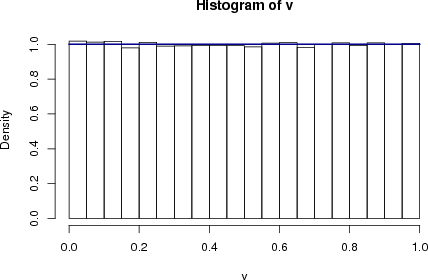
\includegraphics[width=0.7\linewidth]{images/runif-1} 

}

\caption{Simulação de variável com distribuição uniforme}\label{fig:runif}
\end{figure}

\subsubsection{Distribuição normal}\label{distribuicao-normal}

O mesmo procedimento pode ser feito para a distribuição normal, onde
deve-se definir uma valor para a média (\texttt{mean\ =\ 10}) e o
desvio-padrão (\texttt{sd\ =\ 2}) dos dados simulados.

\begin{Shaded}
\begin{Highlighting}[]
\NormalTok{v <-}\StringTok{ }\KeywordTok{rnorm}\NormalTok{(}\DecValTok{10}\OperatorTok{^}\DecValTok{5}\NormalTok{, }\DataTypeTok{mean =} \DecValTok{10}\NormalTok{, }\DataTypeTok{sd =} \DecValTok{2}\NormalTok{)}
\KeywordTok{hist}\NormalTok{(v, }\DataTypeTok{freq =} \OtherTok{FALSE}\NormalTok{)}
\KeywordTok{curve}\NormalTok{(}\KeywordTok{dnorm}\NormalTok{(x, }\DataTypeTok{mean =} \DecValTok{10}\NormalTok{, }\DataTypeTok{sd =} \DecValTok{2}\NormalTok{), }
          \DataTypeTok{col=}\StringTok{"darkblue"}\NormalTok{, }\DataTypeTok{lwd=}\DecValTok{2}\NormalTok{, }\DataTypeTok{add=}\OtherTok{TRUE}\NormalTok{, }\DataTypeTok{yaxt=}\StringTok{"n"}\NormalTok{)}
\end{Highlighting}
\end{Shaded}

\begin{figure}[H]

{\centering 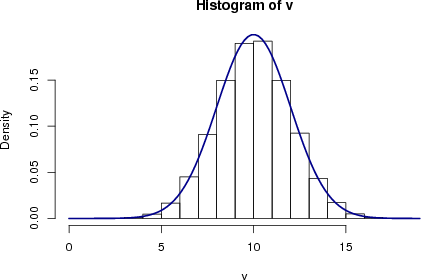
\includegraphics[width=0.7\linewidth]{images/rnorm-1} 

}

\caption{Simulação de variável com distribuição normal}\label{fig:rnorm}
\end{figure}

\subsubsection{Distribuição beta}\label{distribuicao-beta}

Para a geração de variáveis com distribuição beta, basta informa os
parâmetros de forma da mesma, através dos argumentos \texttt{shape1}
e\texttt{shape2}:

\begin{Shaded}
\begin{Highlighting}[]
\NormalTok{v <-}\StringTok{ }\KeywordTok{rbeta}\NormalTok{(}\DecValTok{10}\OperatorTok{^}\DecValTok{5}\NormalTok{, }\DataTypeTok{shape1 =} \DecValTok{4}\NormalTok{, }\DataTypeTok{shape2 =} \DecValTok{4}\NormalTok{)}
\KeywordTok{hist}\NormalTok{(v, }\DataTypeTok{freq =} \OtherTok{FALSE}\NormalTok{)}
\KeywordTok{curve}\NormalTok{(}\KeywordTok{dbeta}\NormalTok{(x, }\DecValTok{4}\NormalTok{, }\DecValTok{4}\NormalTok{), }
          \DataTypeTok{col=}\StringTok{"darkblue"}\NormalTok{, }\DataTypeTok{lwd=}\DecValTok{2}\NormalTok{, }\DataTypeTok{add=}\OtherTok{TRUE}\NormalTok{, }\DataTypeTok{yaxt=}\StringTok{"n"}\NormalTok{)}
\end{Highlighting}
\end{Shaded}

\begin{figure}[H]

{\centering \includegraphics[width=0.7\linewidth]{images/rbeta1-1} 

}

\caption{Simulação de variável com distribuição beta (fatores de forma iguais a 4)}\label{fig:rbeta1}
\end{figure}

No caso da distribuição beta a escolha dos parâmetros deve ser
criteriosa, haja vista que a mesma pode assumir as mais diferentes
formas. Por exemplo, a distribuição beta com parâmetros de forma iguais
a 1 é equivalente à distribuição uniforme

\begin{Shaded}
\begin{Highlighting}[]
\NormalTok{v <-}\StringTok{ }\KeywordTok{rbeta}\NormalTok{(}\DecValTok{10}\OperatorTok{^}\DecValTok{5}\NormalTok{, }\DataTypeTok{shape1 =} \DecValTok{1}\NormalTok{, }\DataTypeTok{shape2 =} \DecValTok{1}\NormalTok{)}
\KeywordTok{hist}\NormalTok{(v, }\DataTypeTok{freq =} \OtherTok{FALSE}\NormalTok{)}
\KeywordTok{curve}\NormalTok{(}\KeywordTok{dunif}\NormalTok{(x),}
          \DataTypeTok{col=}\StringTok{"darkblue"}\NormalTok{, }\DataTypeTok{lwd=}\DecValTok{2}\NormalTok{, }\DataTypeTok{add=}\OtherTok{TRUE}\NormalTok{, }\DataTypeTok{yaxt=}\StringTok{"n"}\NormalTok{)}
\end{Highlighting}
\end{Shaded}

\begin{figure}[H]

{\centering 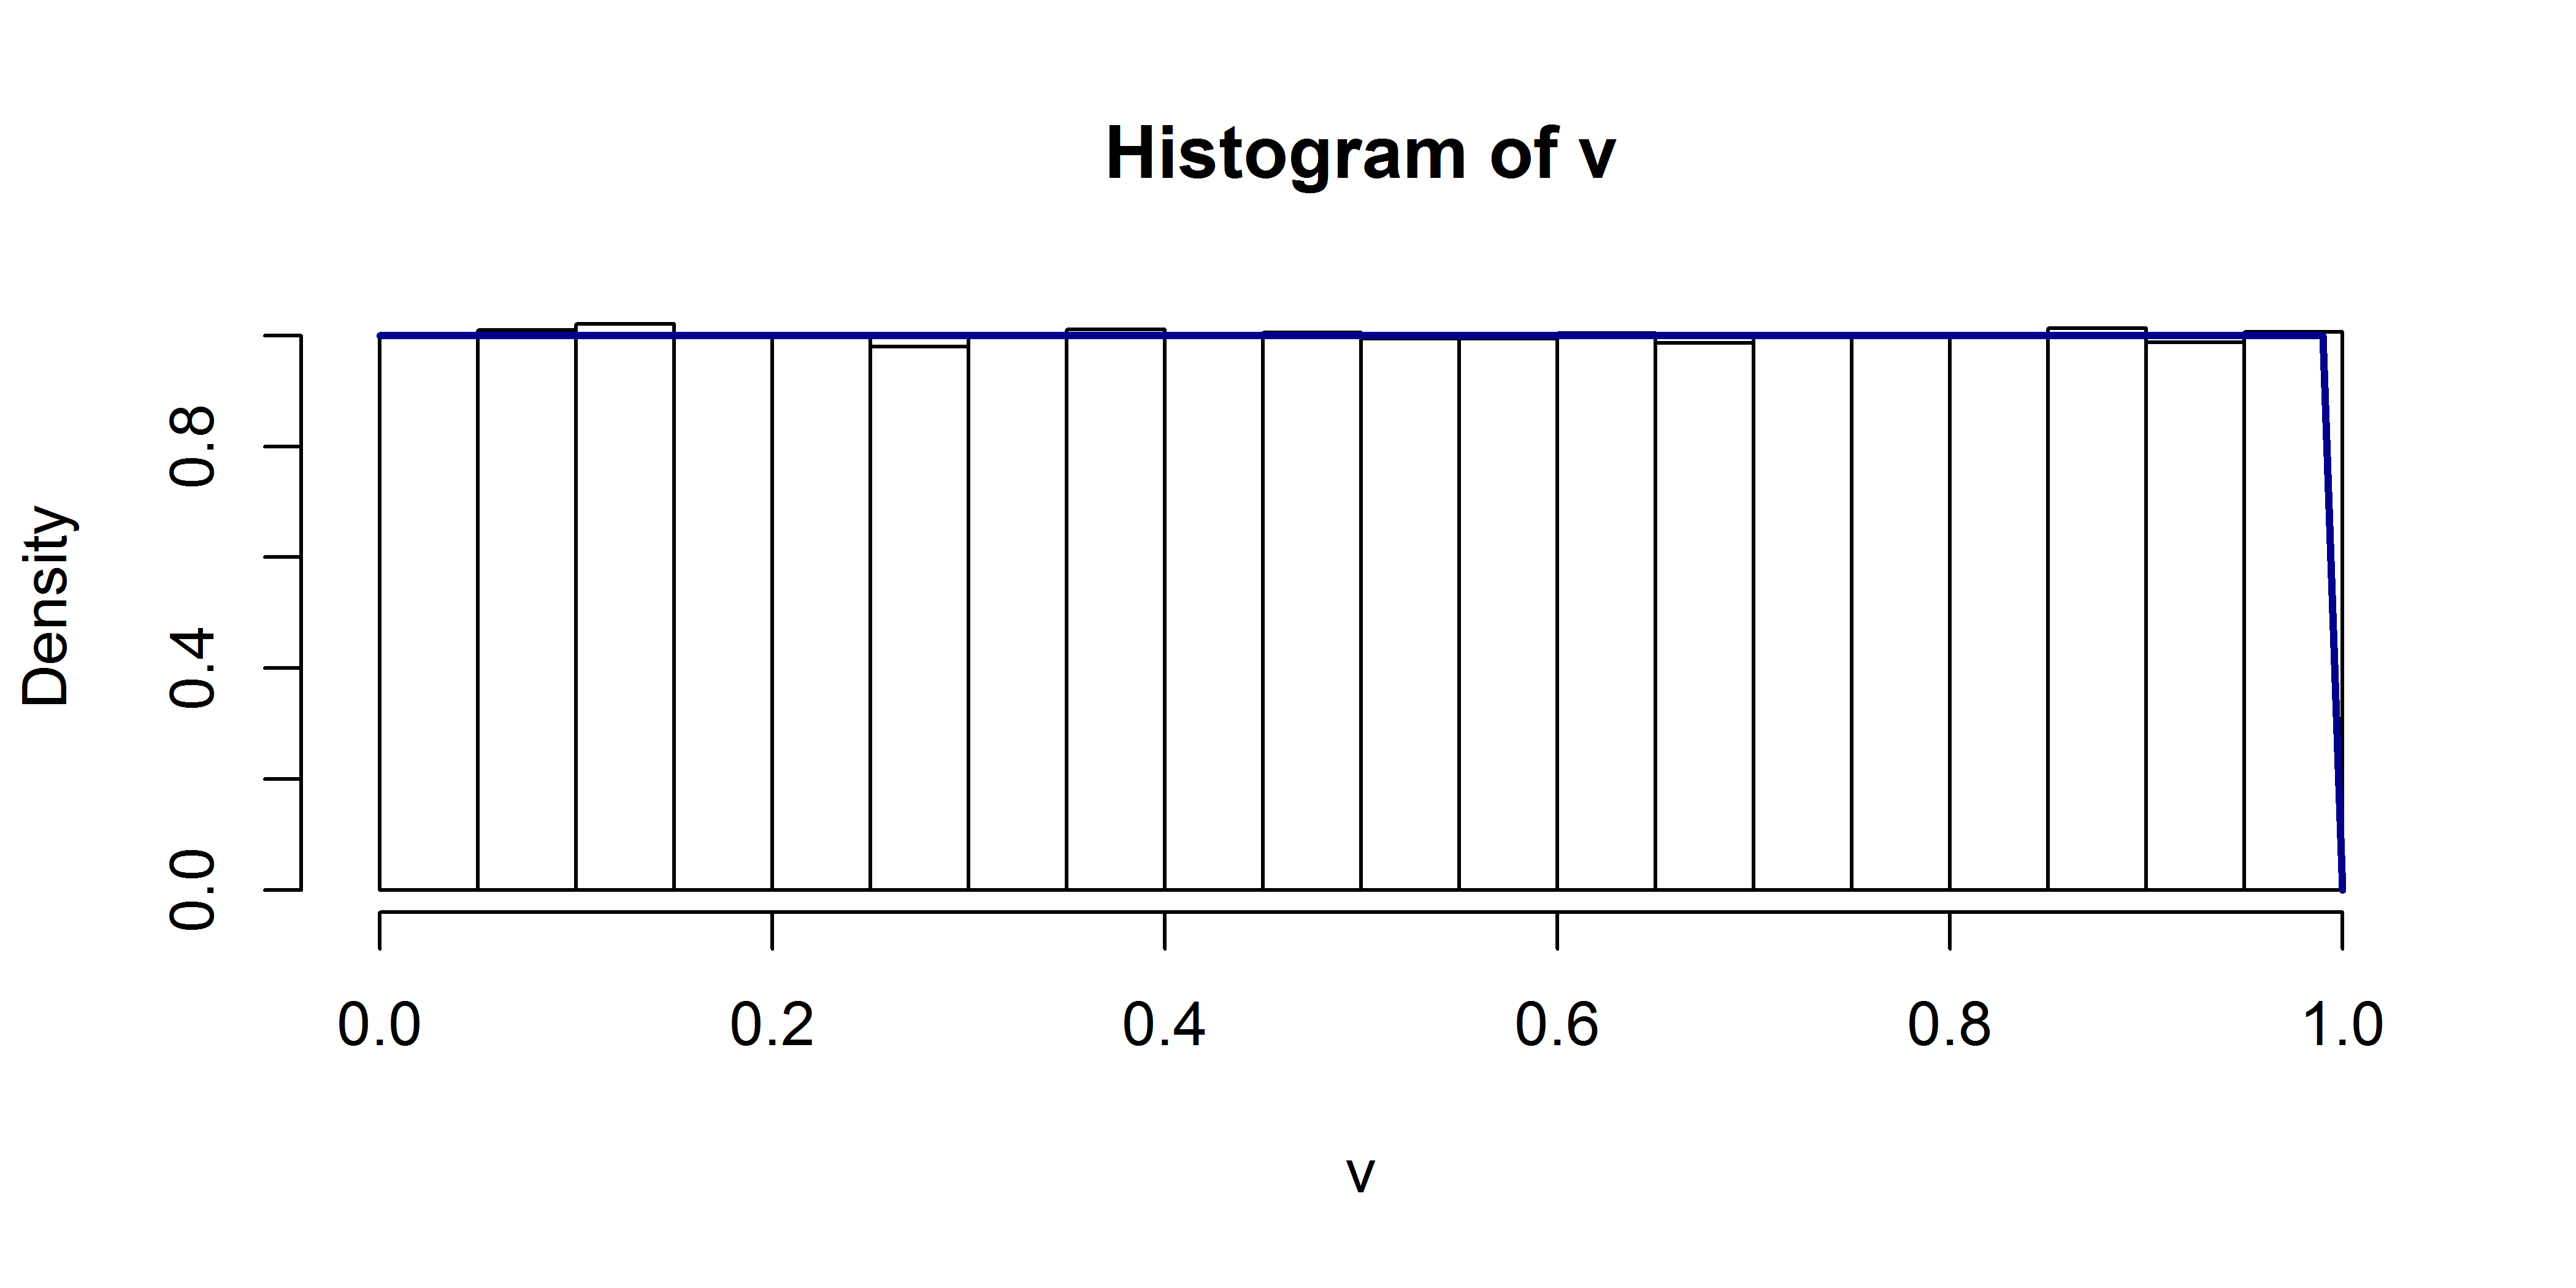
\includegraphics[width=0.7\linewidth]{images/rbeta2-1} 

}

\caption{Simulação de variável com distribuição beta (fatores de forma iguais a 1)}\label{fig:rbeta2}
\end{figure}

\subsection{Geração de variáveis aleatórias
multivariadas}\label{geracao-de-variaveis-aleatorias-multivariadas}

\subsubsection{Distribuição normal
multivariada}\label{distribuicao-normal-multivariada}

Abaixo demonstramos com simular \texttt{n} variáveis aleatórias
\textbf{independentes} de uma distribuição normal multivariada, assim
como obter seus gráficos tridimensionais. Para as simulações podem ser
utilizadas a função \texttt{mvrnorm}, disponível dentro do pacote
\texttt{MASS}(\protect\hyperlink{ref-MASS}{2002}).

\begin{Shaded}
\begin{Highlighting}[]
\KeywordTok{library}\NormalTok{(MASS)}
\CommentTok{# Geração}
\NormalTok{bivn <-}\StringTok{ }\KeywordTok{mvrnorm}\NormalTok{(}\DecValTok{10}\OperatorTok{^}\DecValTok{5}\NormalTok{, }\DataTypeTok{mu =} \KeywordTok{c}\NormalTok{(}\DecValTok{0}\NormalTok{, }\DecValTok{0}\NormalTok{), }\DataTypeTok{Sigma =} \KeywordTok{diag}\NormalTok{(}\DecValTok{2}\NormalTok{))}

\CommentTok{# Gráficos}
\KeywordTok{par}\NormalTok{(}\DataTypeTok{mfrow =} \KeywordTok{c}\NormalTok{(}\DecValTok{2}\NormalTok{, }\DecValTok{3}\NormalTok{))}
\CommentTok{# now we do a kernel density estimate}
\NormalTok{bivn.kde <-}\StringTok{ }\KeywordTok{kde2d}\NormalTok{(bivn[,}\DecValTok{1}\NormalTok{], bivn[,}\DecValTok{2}\NormalTok{], }\DataTypeTok{n =} \DecValTok{50}\NormalTok{)}

\CommentTok{# now plot your results}
\KeywordTok{contour}\NormalTok{(bivn.kde)}
\KeywordTok{image}\NormalTok{(bivn.kde)}

\CommentTok{# fancy contour with image}
\KeywordTok{image}\NormalTok{(bivn.kde); }\KeywordTok{contour}\NormalTok{(bivn.kde, }\DataTypeTok{add =}\NormalTok{ T)}

\CommentTok{# fancy perspectives}
\KeywordTok{persp}\NormalTok{(bivn.kde, }\DataTypeTok{phi =} \DecValTok{45}\NormalTok{, }\DataTypeTok{theta =} \DecValTok{30}\NormalTok{)}
\KeywordTok{persp}\NormalTok{(bivn.kde, }\DataTypeTok{phi =} \DecValTok{45}\NormalTok{, }\DataTypeTok{theta =} \DecValTok{30}\NormalTok{, }\DataTypeTok{shade =}\NormalTok{ .}\DecValTok{1}\NormalTok{, }\DataTypeTok{border =} \OtherTok{NA}\NormalTok{)}
\end{Highlighting}
\end{Shaded}

\begin{figure}[H]

{\centering \includegraphics[width=0.7\linewidth]{images/mvrnorm-1} 

}

\caption{Simulação de variáveis independentes com distribuição normal multivariada}\label{fig:mvrnorm}
\end{figure}

A independência das variáveis foi estabelecida acima através do
argumento \texttt{Sigma} da função \texttt{mvrnorm}, onde estabelecemos
uma matriz diagonal de duas dimensões (\texttt{diag(2)}).

A matriz de covariância dos dados simulados pode ser verificada como
exibimos abaixo:

\begin{Shaded}
\begin{Highlighting}[]
\NormalTok{COV <-}\StringTok{ }\KeywordTok{cov}\NormalTok{(bivn)}
\KeywordTok{row.names}\NormalTok{(COV) <-}\StringTok{ }\KeywordTok{c}\NormalTok{(}\StringTok{"V1"}\NormalTok{, }\StringTok{"V2"}\NormalTok{)}
\KeywordTok{colnames}\NormalTok{(COV) <-}\StringTok{ }\KeywordTok{c}\NormalTok{(}\StringTok{"V1"}\NormalTok{, }\StringTok{"V2"}\NormalTok{)}
\NormalTok{COV }\OperatorTok\StringTok{ }\KeywordTok{kable}\NormalTok{(}\DataTypeTok{format =} \KeywordTok{ifelse}\NormalTok{(type }\OperatorTok{==}\StringTok{ "html"}\NormalTok{, }\StringTok{"markdown"}\NormalTok{, type),}
              \DataTypeTok{caption =} \StringTok{"Matriz de correlação verificada"}\NormalTok{, }
              \DataTypeTok{digits =} \DecValTok{3}\NormalTok{,}
              \DataTypeTok{booktabs =} \OtherTok{TRUE}\NormalTok{) }\OperatorTok
\StringTok{  }\KeywordTok{kable_styling}\NormalTok{(}\DataTypeTok{bootstrap_options =} \StringTok{"striped"}\NormalTok{, }
                \DataTypeTok{full_width =} \OtherTok{FALSE}\NormalTok{)}
\end{Highlighting}
\end{Shaded}

\begin{table}

\caption{\label{tab:cov}Matriz de correlação verificada}
\centering
\begin{tabular}[t]{lrr}
\toprule
  & V1 & V2\\
\midrule
V1 & 0.995 & -0.002\\
V2 & -0.002 & 0.997\\
\bottomrule
\end{tabular}
\end{table}

Para simular \texttt{n} vairáveis aleatórias \textbf{dependentes}, basta
fornecermos uma matriz \texttt{Sigma} simétrica com os termos fora das
diagonais fornecendo o coeficiente de correlação entre elas. Por
exemplo:

\rowcolors{2}{gray!6}{white}

\begin{table}

\caption{\label{tab:simcor}Matriz de covariância desejada entre as variáveis aleatórias}
\centering
\begin{tabular}[t]{lrr}
\hiderowcolors
\toprule
  & V1 & V2\\
\midrule
\showrowcolors
V1 & 1.0 & 0.5\\
V2 & 0.5 & 1.0\\
\bottomrule
\end{tabular}
\end{table}

\rowcolors{2}{white}{white}

\begin{Shaded}
\begin{Highlighting}[]
\CommentTok{# Geração}
\NormalTok{bivn <-}\StringTok{ }\KeywordTok{mvrnorm}\NormalTok{(}\DecValTok{10}\OperatorTok{^}\DecValTok{5}\NormalTok{, }\DataTypeTok{mu =} \KeywordTok{c}\NormalTok{(}\DecValTok{0}\NormalTok{, }\DecValTok{0}\NormalTok{), }\DataTypeTok{Sigma =}\NormalTok{  S)}

\CommentTok{# Gráficos}
\KeywordTok{par}\NormalTok{(}\DataTypeTok{mfrow =} \KeywordTok{c}\NormalTok{(}\DecValTok{2}\NormalTok{, }\DecValTok{3}\NormalTok{))}
\CommentTok{# now we do a kernel density estimate}
\NormalTok{bivn.kde <-}\StringTok{ }\KeywordTok{kde2d}\NormalTok{(bivn[,}\DecValTok{1}\NormalTok{], bivn[,}\DecValTok{2}\NormalTok{], }\DataTypeTok{n =} \DecValTok{50}\NormalTok{)}

\CommentTok{# now plot your results}
\KeywordTok{contour}\NormalTok{(bivn.kde)}
\KeywordTok{image}\NormalTok{(bivn.kde)}

\CommentTok{# fancy contour with image}
\KeywordTok{image}\NormalTok{(bivn.kde); }\KeywordTok{contour}\NormalTok{(bivn.kde, }\DataTypeTok{add =}\NormalTok{ T)}

\CommentTok{# fancy perspectives}
\KeywordTok{persp}\NormalTok{(bivn.kde, }\DataTypeTok{phi =} \DecValTok{45}\NormalTok{, }\DataTypeTok{theta =} \DecValTok{30}\NormalTok{)}
\KeywordTok{persp}\NormalTok{(bivn.kde, }\DataTypeTok{phi =} \DecValTok{45}\NormalTok{, }\DataTypeTok{theta =} \DecValTok{30}\NormalTok{, }\DataTypeTok{shade =}\NormalTok{ .}\DecValTok{1}\NormalTok{, }\DataTypeTok{border =} \OtherTok{NA}\NormalTok{)}
\end{Highlighting}
\end{Shaded}

\begin{figure}[H]

{\centering 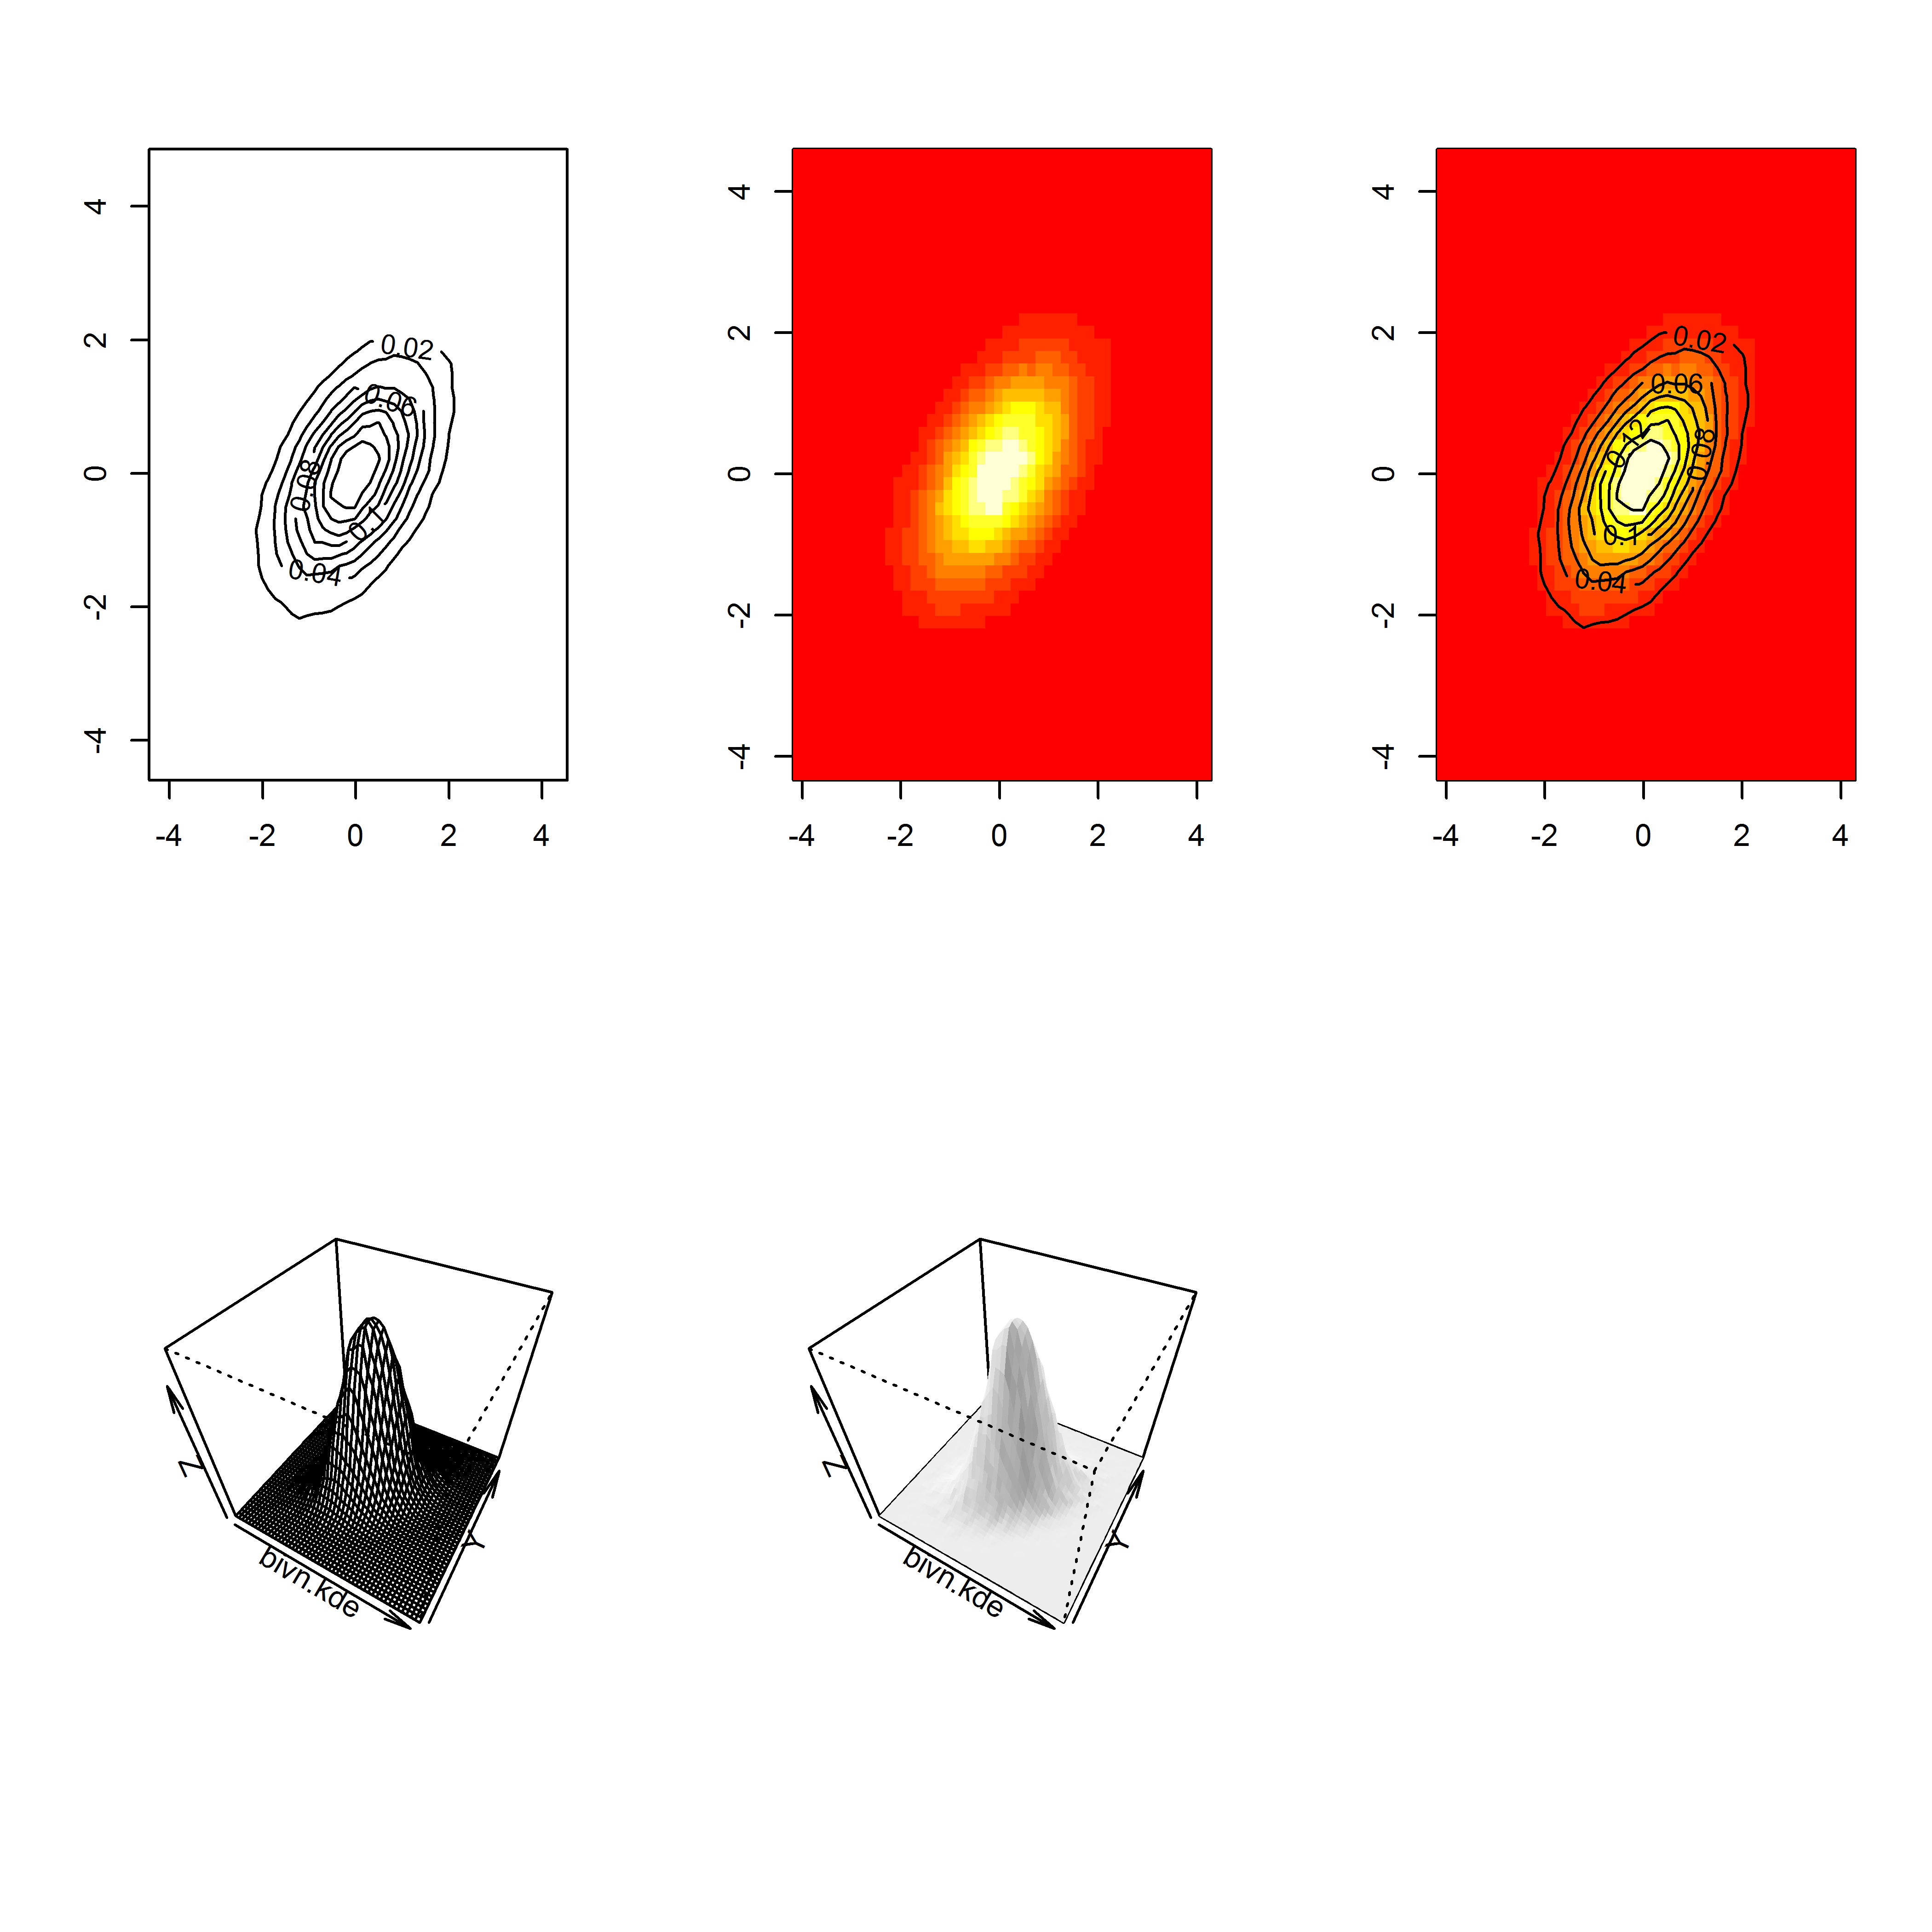
\includegraphics[width=0.7\linewidth]{images/mvnormdep-1} 

}

\caption{Simulação de variáveis dependentes ($\rho = 0,5$) com distribuição normal multivariada}\label{fig:mvnormdep}
\end{figure}

\subsubsection{Distribuição de
Dirichlet}\label{distribuicao-de-dirichlet}

A simulação de dados multivariados da distribuição de Dirichlet, que é
uma versão generalização multivariada da distribuição beta, pode ser
feita através da função \texttt{rdirichlet}, do pacote
\texttt{LearnBayes}(ALBERT, \protect\hyperlink{ref-LearnBayes}{2014}):

\begin{Shaded}
\begin{Highlighting}[]
\CommentTok{# Geração}
\NormalTok{m <-}\StringTok{ }\KeywordTok{rdirichlet}\NormalTok{(}\DecValTok{10}\OperatorTok{^}\DecValTok{2}\NormalTok{, }\DataTypeTok{par =} \KeywordTok{c}\NormalTok{(}\DecValTok{1}\NormalTok{, }\DecValTok{1}\NormalTok{))}
\NormalTok{dir.kde <-}\StringTok{ }\KeywordTok{kde2d}\NormalTok{(m[,}\DecValTok{1}\NormalTok{], m[,}\DecValTok{2}\NormalTok{], }\DataTypeTok{n =} \DecValTok{50}\NormalTok{)}

\CommentTok{# Gráficos}
\KeywordTok{par}\NormalTok{(}\DataTypeTok{mfrow =} \KeywordTok{c}\NormalTok{(}\DecValTok{2}\NormalTok{, }\DecValTok{3}\NormalTok{))}
\CommentTok{# now plot your results}
\KeywordTok{contour}\NormalTok{(dir.kde)}
\KeywordTok{image}\NormalTok{(dir.kde)}
\KeywordTok{persp}\NormalTok{(dir.kde, }\DataTypeTok{phi =} \DecValTok{45}\NormalTok{, }\DataTypeTok{theta =} \DecValTok{30}\NormalTok{)}

\CommentTok{# fancy contour with image}
\KeywordTok{image}\NormalTok{(dir.kde); }\KeywordTok{contour}\NormalTok{(dir.kde, }\DataTypeTok{add =}\NormalTok{ T)}

\CommentTok{# fancy perspective}
\KeywordTok{persp}\NormalTok{(dir.kde, }\DataTypeTok{phi =} \DecValTok{45}\NormalTok{, }\DataTypeTok{theta =} \DecValTok{30}\NormalTok{, }\DataTypeTok{shade =}\NormalTok{ .}\DecValTok{1}\NormalTok{, }\DataTypeTok{border =} \OtherTok{NA}\NormalTok{)}
\end{Highlighting}
\end{Shaded}

\begin{figure}[H]

{\centering 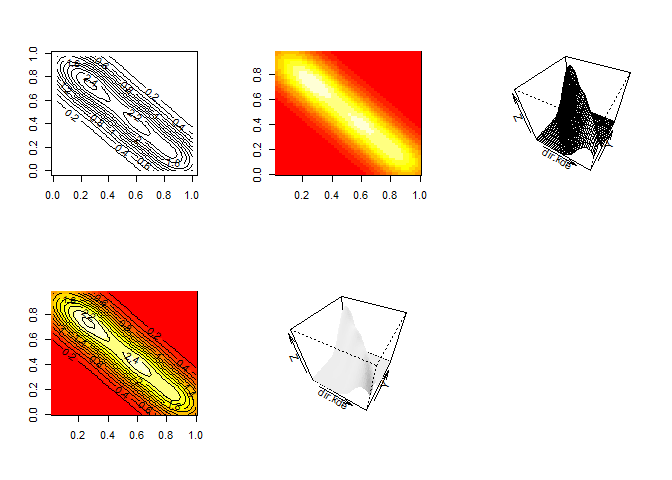
\includegraphics[width=0.7\linewidth]{images/dirichlet-1} 

}

\caption{Simulação de distribuição Dirichlet - parâmetros iguais a 1}\label{fig:dirichlet}
\end{figure}

\subsubsection{Simulação de variáveis aleatórias dependentes usando
Copulas}\label{simulacao-de-variaveis-aleatorias-dependentes-usando-copulas}

Para a simulação de variáveis dependentes de quaisquer distribuições, a
utilização do Método Copulas é interessante. Há alguns pacotes que
implementam este método, como o pacote \texttt{simstudy}{[}-simstudy{]},
cuja utilização para o método Copulas pode ser vista em GOLDFELD
(\protect\hyperlink{ref-Copulas}{2017}). Mas o método também pode ser
facilmente implementado com as funções básicas apresentadas até aqui(ver
SMART, \protect\hyperlink{ref-econometrics}{2014}).

O método consiste em primeiramente gerar \texttt{n} variaveis aleatórias
dependentes com a função normal multivariada, transformar estas
variáveis brutas em \texttt{n} vetores de probabilidades normal através
da função \texttt{pnorm} e finalmente transformar estes vetores de
probabilidades normais em vetores de quantis da distribuição desejada.

Uma versão personalizada deste método com foco na aplicação do Método de
Monte Carlo à avaliação de imóveis pelo método involutivo foi elaborada
por este autor e encontra-se disponível através da função
\texttt{vpl\_sim} do pacote \texttt{appraiseR}\footnote{Ver
  \url{https://github.com/lfpdroubi/appraiseR}}(DROUBI,
\protect\hyperlink{ref-appraiseR}{2018}).

\section{Estudo de Caso}\label{estudo-de-caso}

\subsection{Dados Preliminares}\label{dados-preliminares}

Trata-se de avaliar pelo método involutivo um terreno com área de 500
m\^{}2, cujos estudos de mercado indicam que o melhor aproveitamento
para este terreno é a construção de um prédio residencial.
Considerando-se o máximo aproveitamento possível (o índice de
aproveitamento do terreno é 2.5), pode-se construir 20 apartamentos com
área total de 75 m\^{}2 cada um, num prédio de 6 pisos (5 + 1).

\subsection{Previsão de Receitas ou Valor Global de Vendas (VGV) e
velocidade de
vendas}\label{previsao-de-receitas-ou-valor-global-de-vendas-vgv-e-velocidade-de-vendas}

O Produto Geral de Vendas (Pgv) ou Valor Global de Vendas (VGV) é o
Produto de vendas total do empreendimento hipotético.

O preço de venda praticado pelo mercado na região do imóvel é de R\$
7.000,00/ m\^{}2, o que gera um vgv de R\$ 10.500.000,00.

Já o cronograma de venda foi estimado bimestralmente como mostrado
abaixo:

\begin{table}

\caption{\label{tab:wv}Vendas por período}
\centering
\begin{tabular}[t]{lllllllllllllll}
\toprule
Periodo & 0 & 1 & 2 & 3 & 4 & 5 & 6 & 7 & 8 & 9 & 10 & 11 & 12 & 13\\
Vendas & 0\% & 0\% & 5\% & 5\% & 5\% & 5\% & 10\% & 10\% & 10\% & 10\% & 10\% & 10\% & 10\% & 10\%\\
\bottomrule
\end{tabular}
\end{table}

\subsection{Custos de Construção e Cronograma
Financeiro}\label{custos-de-construcao-e-cronograma-financeiro}

Estima-se que o custo de construção seja 120\% do CUB R8N, que no
momento é de R\$ 1.553,57/ m\^{}2, de maneira então que o custo de
referência será de R\$ 1.864,28/ m\^{}2, totalizando R\$ 2.796.426,00.

O cronograma financeiro da construção foi estimado bimestralmente como
mostrado a baixo:

\begin{table}

\caption{\label{tab:wc}Cronograma financeiro -- Custos de Construção}
\centering
\begin{tabular}[t]{lllllllllll}
\toprule
Periodo & 0 & 1 & 2 & 3 & 4 & 5 & 6 & 7 & 8 & 9\\
Custos & 5.67\% & 6.63\% & 7.24\% & 7.55\% & 10.76\% & 13.26\% & 14.72\% & 13.16\% & 14.18\% & 6.84\%\\
\bottomrule
\end{tabular}
\end{table}

\subsection{Taxa mínima de atratividade
(TMA)}\label{taxa-minima-de-atratividade-tma}

A taxa mínima de atratividade do empreendimento foi calculada levando em
consideração a taxa livre de risco do mercado, atualmente em 1,20\% a.b.
e a taxa de risco do empreendimento, adotada 0,70\% a.b., resultando
numa TMA de 1,91\% a.b..

\hypertarget{fluxo-de-caixa-provavel-do-empreendimento}{\subsection{Fluxo
de Caixa Provável do
Empreendimento}\label{fluxo-de-caixa-provavel-do-empreendimento}}

O Fluxo de Caixa do Empreendimento pode ser visto abaixo:

\rowcolors{2}{gray!6}{white}

\begin{table}

\caption{\label{tab:FC}Tabela de Fluxo de Caixa do Emprendimento}
\centering
\resizebox{\linewidth}{!}{\begin{tabular}[t]{rrrrrrrr}
\hiderowcolors
\toprule
Periodo & FCV & FCI & Corretagem & BDI\_Incorporador & FCL & fator\_VP & FCL\_descontado\\
\midrule
\showrowcolors
0 & 0 & -208.439,5 & 0 & 0 & -208.439,50 & 1,00 & -208.439,50\\
1 & 0 & -243.730,8 & 0 & 0 & -243.730,84 & 0,98 & -239.166,59\\
2 & 525.000 & -266.155,5 & -26.250 & -123.480 & 109.114,45 & 0,96 & 105.066,03\\
3 & 525.000 & -277.551,7 & -26.250 & -123.480 & 97.718,29 & 0,94 & 92.330,65\\
4 & 525.000 & -395.557,1 & -26.250 & -123.480 & -20.287,14 & 0,93 & -18.809,66\\
\addlinespace
5 & 525.000 & -487.461,7 & -26.250 & -123.480 & -112.191,68 & 0,91 & -102.072,97\\
6 & 1.050.000 & -541.133,9 & -52.500 & -246.960 & 209.406,07 & 0,89 & 186.951,67\\
7 & 1.050.000 & -483.785,5 & -52.500 & -246.960 & 266.754,50 & 0,88 & 233.690,94\\
8 & 1.050.000 & -521.282,5 & -52.500 & -246.960 & 229.257,45 & 0,86 & 197.080,47\\
9 & 1.050.000 & -251.450,8 & -52.500 & -246.960 & 499.089,18 & 0,84 & 421.006,02\\
\addlinespace
10 & 1.050.000 & 0,0 & -52.500 & -246.960 & 750.540,00 & 0,83 & 621.260,89\\
11 & 1.050.000 & 0,0 & -52.500 & -246.960 & 750.540,00 & 0,81 & 609.626,77\\
12 & 1.050.000 & 0,0 & -52.500 & -246.960 & 750.540,00 & 0,80 & 598.210,52\\
13 & 1.050.000 & 0,0 & -52.500 & -246.960 & 750.540,00 & 0,78 & 587.008,06\\
\bottomrule
\end{tabular}}
\end{table}

\rowcolors{2}{white}{white}

\subsection{Valor Presente Líquido (VPL)
Provável}\label{valor-presente-liquido-vpl-provavel}

De acordo com o observado no fluxo de caixa acima, o VPL do
empreendimento é a soma da coluna do Fluxo de Caixa Líquido descontado
-- da taxa de juros mínima de atratividade, ou seja, o VPL é \textbf{R\$
3.083.743,30}.

\subsection{Análises de Sensibilidade}\label{analises-de-sensibilidade}

\subsubsection{Sensibilidade em relação à taxa mínima de
atratividade}\label{sensibilidade-em-relacao-a-taxa-minima-de-atratividade}

Em relação à taxa mínima de atratividade (TMA), a consideraremos
variando entre o valor mínimo de 1,20\% a.b. para o cenário otimista e o
valor máximo de 2,60\% a.b., no cenário pessimista.

\rowcolors{2}{gray!6}{white}

\begin{table}

\caption{\label{tab:s_tma}Sensibilidade do VPL à variação da TMA}
\centering
\begin{tabular}[t]{lrrr}
\hiderowcolors
\toprule
Situacao & TMA & VPL & Variacao\\
\midrule
\showrowcolors
Pessimista & 0,026 & 2.852.118 & -0,076\\
Provavel & 0,019 & 3.086.672 & 0,000\\
Otimista & 0,012 & 3.341.070 & 0,082\\
\bottomrule
\end{tabular}
\end{table}

\rowcolors{2}{white}{white}

\subsubsection{Sensibilidade em relação ao custo de construção do
empreendimento}\label{sensibilidade-em-relacao-ao-custo-de-construcao-do-empreendimento}

Em relação ao custo do empreendimento, consideraremos uma variação no
custo de construção (antes do BDI do construtor) entre 90\% e 110\% do
custo provável.

\rowcolors{2}{gray!6}{white}

\begin{table}

\caption{\label{tab:s_custo}Sensibilidade do VPL à variação do Custo de Construção}
\centering
\begin{tabular}[t]{lrrr}
\hiderowcolors
\toprule
Situacao & CC & VPL & Variacao\\
\midrule
\showrowcolors
Pessimista & 2.516.783 & 3.418.098 & 0,11\\
Provavel & 2.796.426 & 3.083.743 & 0,00\\
Otimista & 3.076.069 & 2.749.389 & -0,11\\
\bottomrule
\end{tabular}
\end{table}

\rowcolors{2}{white}{white}

\subsubsection{Sensibilidade em relação ao BDI do
Construtor}\label{sensibilidade-em-relacao-ao-bdi-do-construtor}

Em relação ao BDI do Construtor, consideraremos uma variação entre 90\%
e 110\% do BDI provável.

\rowcolors{2}{gray!6}{white}

\begin{table}

\caption{\label{tab:s_bdi_c}Sensibilidade do VPL à variação do BDI do Construtor}
\centering
\begin{tabular}[t]{lrrr}
\hiderowcolors
\toprule
Situacao & BDI\_Construtor & VPL & Variacao\\
\midrule
\showrowcolors
Pessimista & 0,35 & 3.003.728 & -0,03\\
Provavel & 0,31 & 3.083.743 & 0,00\\
Otimista & 0,28 & 3.163.758 & 0,03\\
\bottomrule
\end{tabular}
\end{table}

\rowcolors{2}{white}{white}

\subsubsection{Sensibilidade em relação ao valor de venda do
empreendimento}\label{sensibilidade-em-relacao-ao-valor-de-venda-do-empreendimento}

Em relação às vendas, consideraremos uma variação entre 90\% e 110\% do
vgv provável.

\rowcolors{2}{gray!6}{white}

\begin{table}

\caption{\label{tab:s_vgv}Sensibilidade do VPL à variação do VGV}
\centering
\begin{tabular}[t]{lrrr}
\hiderowcolors
\toprule
Situacao & Vendas & VPL & Variacao\\
\midrule
\showrowcolors
Pessimista & 9.450.000 & 2.441.015 & -0,21\\
Provavel & 10.500.000 & 3.083.743 & 0,00\\
Otimista & 11.550.000 & 3.726.472 & 0,21\\
\bottomrule
\end{tabular}
\end{table}

\rowcolors{2}{white}{white}

\subsubsection{Sensibilidade em relação ao BDI do
Incorporador}\label{sensibilidade-em-relacao-ao-bdi-do-incorporador}

Em relação ao BDI do Incorporador, consideraremos uma variação entre
90\textasciitilde{}\% e 110\% do BDI provável.

\rowcolors{2}{gray!6}{white}

\begin{table}

\caption{\label{tab:s_bdi_i}Sensibilidade do VPL à variação do BDI do Incorporador}
\centering
\begin{tabular}[t]{lrrr}
\hiderowcolors
\toprule
Situacao & BDI\_Incorporador & VPL & Variacao\\
\midrule
\showrowcolors
Pessimista & 0,26 & 2.872.258 & -0,07\\
Provavel & 0,24 & 3.083.743 & 0,00\\
Otimista & 0,21 & 3.295.229 & 0,07\\
\bottomrule
\end{tabular}
\end{table}

\rowcolors{2}{white}{white}

\hypertarget{sensibilidade-em-relacao-a-velocidade-de-vendas-do-empreendimento}{\subsection{Sensibilidade
em relação à velocidade de vendas do
empreendimento}\label{sensibilidade-em-relacao-a-velocidade-de-vendas-do-empreendimento}}

Quanto à velocidade de vendas, consideraremos que as vendas podem ser
feitas, num cenário pessimista, na seguinte velocidade:

\begin{longtable}[]{@{}cccccccccccccc@{}}
\caption{Velocidade de Vendas -- Cenário Pessimista (continued
below)}\tabularnewline
\toprule
\begin{minipage}[t]{0.12\columnwidth}\centering\strut
\textbf{Periodo}\strut
\end{minipage} & \begin{minipage}[t]{0.04\columnwidth}\centering\strut
0\strut
\end{minipage} & \begin{minipage}[t]{0.04\columnwidth}\centering\strut
1\strut
\end{minipage} & \begin{minipage}[t]{0.04\columnwidth}\centering\strut
2\strut
\end{minipage} & \begin{minipage}[t]{0.04\columnwidth}\centering\strut
3\strut
\end{minipage} & \begin{minipage}[t]{0.04\columnwidth}\centering\strut
4\strut
\end{minipage} & \begin{minipage}[t]{0.04\columnwidth}\centering\strut
5\strut
\end{minipage} & \begin{minipage}[t]{0.04\columnwidth}\centering\strut
6\strut
\end{minipage} & \begin{minipage}[t]{0.04\columnwidth}\centering\strut
7\strut
\end{minipage} & \begin{minipage}[t]{0.04\columnwidth}\centering\strut
8\strut
\end{minipage} & \begin{minipage}[t]{0.04\columnwidth}\centering\strut
9\strut
\end{minipage} & \begin{minipage}[t]{0.04\columnwidth}\centering\strut
10\strut
\end{minipage} & \begin{minipage}[t]{0.04\columnwidth}\centering\strut
11\strut
\end{minipage} & \begin{minipage}[t]{0.04\columnwidth}\centering\strut
12\strut
\end{minipage}\tabularnewline
\begin{minipage}[t]{0.12\columnwidth}\centering\strut
\textbf{Vendas}\strut
\end{minipage} & \begin{minipage}[t]{0.04\columnwidth}\centering\strut
0\%\strut
\end{minipage} & \begin{minipage}[t]{0.04\columnwidth}\centering\strut
0\%\strut
\end{minipage} & \begin{minipage}[t]{0.04\columnwidth}\centering\strut
5\%\strut
\end{minipage} & \begin{minipage}[t]{0.04\columnwidth}\centering\strut
5\%\strut
\end{minipage} & \begin{minipage}[t]{0.04\columnwidth}\centering\strut
5\%\strut
\end{minipage} & \begin{minipage}[t]{0.04\columnwidth}\centering\strut
5\%\strut
\end{minipage} & \begin{minipage}[t]{0.04\columnwidth}\centering\strut
5\%\strut
\end{minipage} & \begin{minipage}[t]{0.04\columnwidth}\centering\strut
5\%\strut
\end{minipage} & \begin{minipage}[t]{0.04\columnwidth}\centering\strut
5\%\strut
\end{minipage} & \begin{minipage}[t]{0.04\columnwidth}\centering\strut
5\%\strut
\end{minipage} & \begin{minipage}[t]{0.04\columnwidth}\centering\strut
5\%\strut
\end{minipage} & \begin{minipage}[t]{0.04\columnwidth}\centering\strut
5\%\strut
\end{minipage} & \begin{minipage}[t]{0.04\columnwidth}\centering\strut
5\%\strut
\end{minipage}\tabularnewline
\bottomrule
\end{longtable}

\begin{longtable}[]{@{}cccccccccc@{}}
\toprule
\begin{minipage}[t]{0.14\columnwidth}\centering\strut
\textbf{Periodo}\strut
\end{minipage} & \begin{minipage}[t]{0.05\columnwidth}\centering\strut
13\strut
\end{minipage} & \begin{minipage}[t]{0.05\columnwidth}\centering\strut
14\strut
\end{minipage} & \begin{minipage}[t]{0.05\columnwidth}\centering\strut
15\strut
\end{minipage} & \begin{minipage}[t]{0.05\columnwidth}\centering\strut
16\strut
\end{minipage} & \begin{minipage}[t]{0.05\columnwidth}\centering\strut
17\strut
\end{minipage} & \begin{minipage}[t]{0.05\columnwidth}\centering\strut
18\strut
\end{minipage} & \begin{minipage}[t]{0.05\columnwidth}\centering\strut
19\strut
\end{minipage} & \begin{minipage}[t]{0.05\columnwidth}\centering\strut
20\strut
\end{minipage} & \begin{minipage}[t]{0.05\columnwidth}\centering\strut
21\strut
\end{minipage}\tabularnewline
\begin{minipage}[t]{0.14\columnwidth}\centering\strut
\textbf{Vendas}\strut
\end{minipage} & \begin{minipage}[t]{0.05\columnwidth}\centering\strut
5\%\strut
\end{minipage} & \begin{minipage}[t]{0.05\columnwidth}\centering\strut
5\%\strut
\end{minipage} & \begin{minipage}[t]{0.05\columnwidth}\centering\strut
5\%\strut
\end{minipage} & \begin{minipage}[t]{0.05\columnwidth}\centering\strut
5\%\strut
\end{minipage} & \begin{minipage}[t]{0.05\columnwidth}\centering\strut
5\%\strut
\end{minipage} & \begin{minipage}[t]{0.05\columnwidth}\centering\strut
5\%\strut
\end{minipage} & \begin{minipage}[t]{0.05\columnwidth}\centering\strut
5\%\strut
\end{minipage} & \begin{minipage}[t]{0.05\columnwidth}\centering\strut
5\%\strut
\end{minipage} & \begin{minipage}[t]{0.05\columnwidth}\centering\strut
5\%\strut
\end{minipage}\tabularnewline
\bottomrule
\end{longtable}

Já para o cenário otimista em relação à velocidade de vendas, foi
considerada a seguinte hipótese:

\begin{table}

\caption{\label{tab:wv_otimista}Velocidade de Vendas -- Cenário Otimista}
\centering
\begin{tabular}[t]{lllllllllllll}
\toprule
Periodo & 0 & 1 & 2 & 3 & 4 & 5 & 6 & 7 & 8 & 9 & 10 & 11\\
Vendas & 0\% & 0\% & 10\% & 10\% & 10\% & 10\% & 10\% & 10\% & 10\% & 10\% & 10\% & 10\%\\
\bottomrule
\end{tabular}
\end{table}

\rowcolors{2}{gray!6}{white}

\begin{table}

\caption{\label{tab:s_vv}Sensibilidade do VPL à variação da velocidade de vendas do Empreendimento}
\centering
\begin{tabular}[t]{llrr}
\hiderowcolors
\toprule
Situacao & VV & VPL & Variacao\\
\midrule
\showrowcolors
Pessimista & Pessimista & 2.731.317 & -0,11\\
Provavel & Provavel & 3.083.743 & 0,00\\
Otimista & Otimista & 3.303.815 & 0,07\\
\bottomrule
\end{tabular}
\end{table}

\rowcolors{2}{white}{white}

\subsubsection{Análise gráfica de
sensibilidade}\label{analise-grafica-de-sensibilidade}

Na figura \ref{s_plots} são mostrados os gráficos para as análises de
sensibilidade efetuadas acima.

\begin{figure}[p]

{\centering 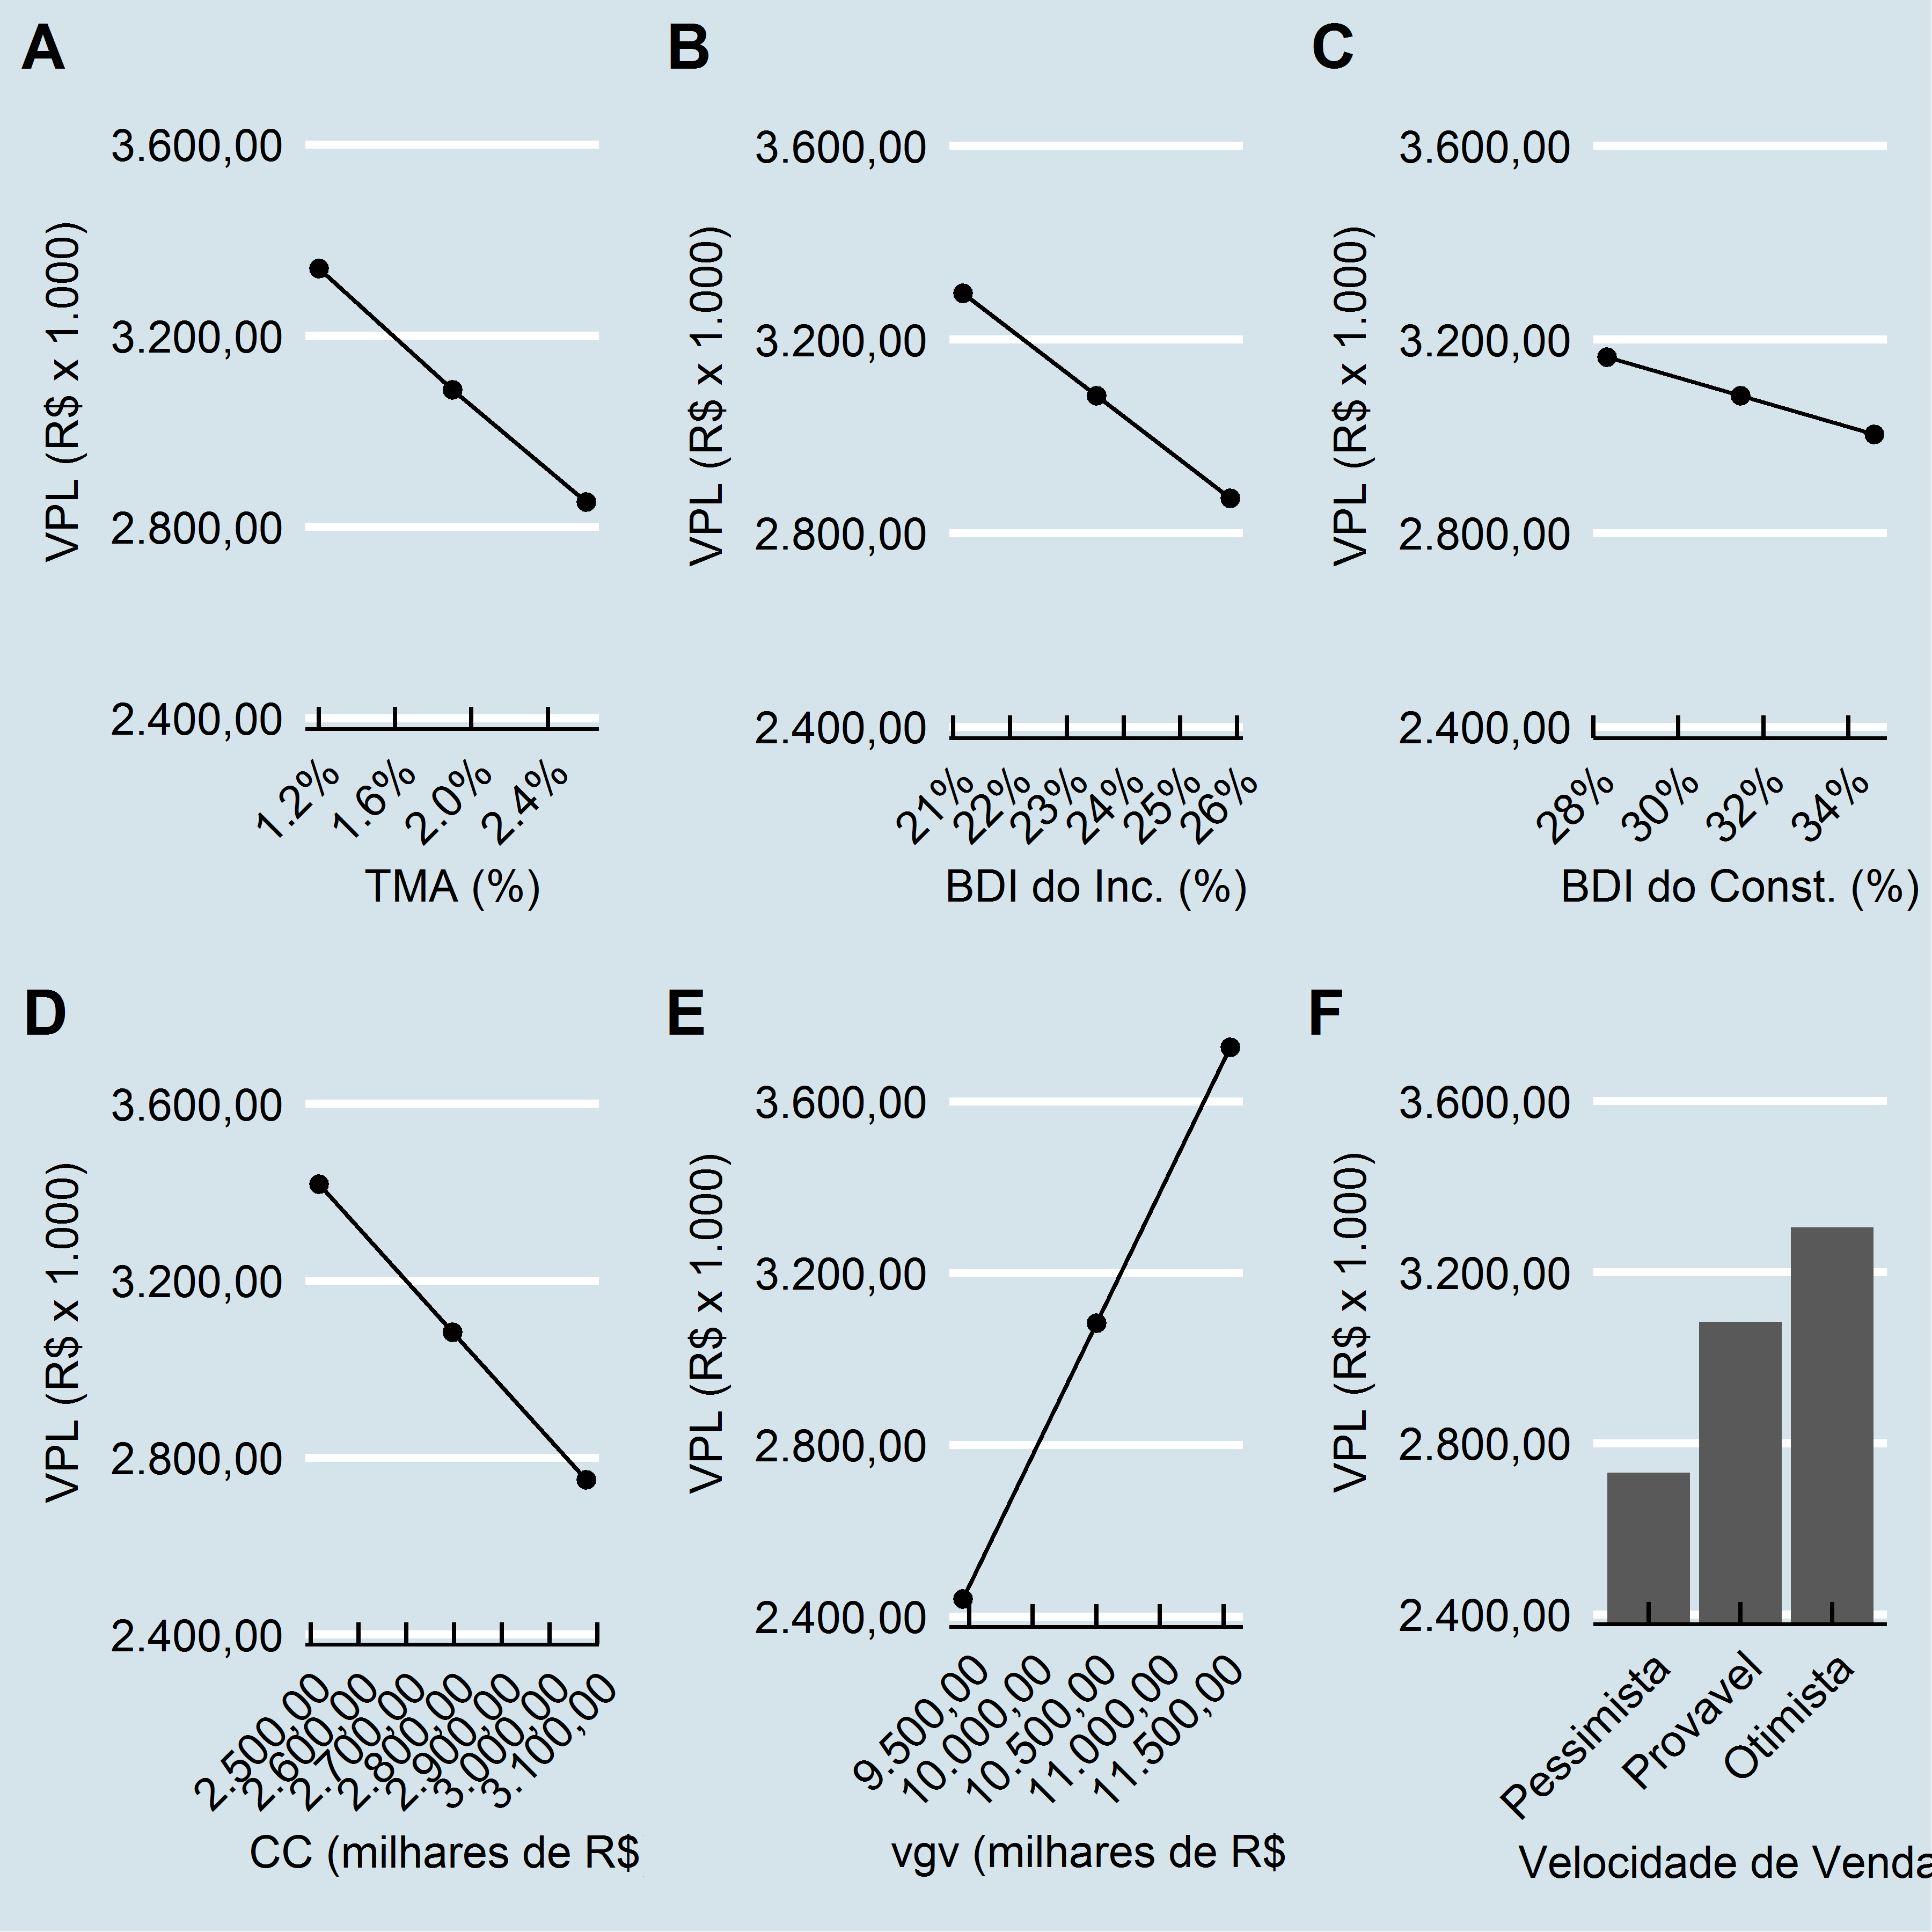
\includegraphics[width=0.7\linewidth]{images/s_plots-1} 

}

\caption{\label{s_plots}Análise de Sensibilidade Gráfica}\label{fig:s_plots}
\end{figure}

Com os gráficos alinhados, e todos com os mesmos limites de escala em
relação ao VPL, é fácil perceber a maior ou menor influência das
diferentes variáveis na composição final do VPL.

Nota-se que, para esta análise, a variação do VGV -- ou melhor, uma
variação no valor unitário de venda -- tem um maior impacto

\subsection{Análise de Cenários}\label{analise-de-cenarios}

Foram analisados três cenários: o pessimista, o mais provável e o
otimista.

Para cada cenário foi calculado um Fluxo de Caixa de Vendas, um Fluxo de
Caixa de Investimentos e um Fluxo de Caixa Líquido, de onde foram
obtidos os VPL's para cada cenário.

\subsubsection{Cenário Pessimista}\label{cenario-pessimista}

No cenário pessimista, o Fluxo de Caixa de Vendas foi elaborado
considerando-se um valor de 90\% do VGV Provável, em conjunto com o
fluxo de vendas pessimista, como pode ser visto em
\protect\hyperlink{sensibilidade-em-relacao-a-velocidade-de-vendas-do-empreendimento}{Sensibilidade
em relação à velocidade de vendas do empreendimento}. Já o Fluxo de
Caixa de Investimentos foi calculado considerando-se o valor de 110\% do
Custo de Construção Provável e com BDI do Construtor com valor de 110\%
do BDI Provável do Construtor. Finalmente, para o Fluxo de Caixa
Líquido, foi considerado um valor de 110\% do BDI Provável do
Incorporador e uma taxa mínima de atratividade de 2.6\%.

\rowcolors{2}{gray!6}{white}

\begin{table}

\caption{\label{tab:pessimista}Fluxo de Caixa Pessimista do Empreendimento}
\centering
\begin{tabu} to \linewidth {>{\raggedleft}X>{\raggedleft}X>{\raggedleft}X>{\raggedleft}X>{\raggedleft}X>{\raggedleft}X>{\raggedleft}X>{\raggedleft}X}
\hiderowcolors
\toprule
Periodo & FCV & FCI & Corretagem & BDI\_Incorporador & FCL & fator\_VP & FCL\_descontado\\
\midrule
\showrowcolors
0 & 0 & -234.770 & 0 & 0 & -234.770 & 1,00 & -234.770\\
1 & 0 & -274.520 & 0 & 0 & -274.520 & 0,97 & -267.563\\
2 & 472.500 & -299.777 & -23.625 & -122.245 & 26.852 & 0,95 & 25.509\\
3 & 472.500 & -312.613 & -23.625 & -122.245 & 14.017 & 0,93 & 12.978\\
4 & 472.500 & -445.526 & -23.625 & -122.245 & -118.896 & 0,90 & -107.294\\
\addlinespace
5 & 472.500 & -549.040 & -23.625 & -122.245 & -222.410 & 0,88 & -195.622\\
6 & 472.500 & -609.492 & -23.625 & -122.245 & -282.863 & 0,86 & -242.489\\
7 & 472.500 & -544.899 & -23.625 & -122.245 & -218.270 & 0,84 & -182.373\\
8 & 472.500 & -587.133 & -23.625 & -122.245 & -260.503 & 0,81 & -212.146\\
9 & 472.500 & -283.215 & -23.625 & -122.245 & 43.415 & 0,79 & 34.460\\
\addlinespace
10 & 472.500 & 0 & -23.625 & -122.245 & 326.630 & 0,77 & 252.687\\
11 & 472.500 & 0 & -23.625 & -122.245 & 326.630 & 0,75 & 246.283\\
12 & 472.500 & 0 & -23.625 & -122.245 & 326.630 & 0,73 & 240.042\\
13 & 472.500 & 0 & -23.625 & -122.245 & 326.630 & 0,72 & 233.959\\
14 & 472.500 & 0 & -23.625 & -122.245 & 326.630 & 0,70 & 228.030\\
\addlinespace
15 & 472.500 & 0 & -23.625 & -122.245 & 326.630 & 0,68 & 222.252\\
16 & 472.500 & 0 & -23.625 & -122.245 & 326.630 & 0,66 & 216.620\\
17 & 472.500 & 0 & -23.625 & -122.245 & 326.630 & 0,65 & 211.130\\
18 & 472.500 & 0 & -23.625 & -122.245 & 326.630 & 0,63 & 205.780\\
19 & 472.500 & 0 & -23.625 & -122.245 & 326.630 & 0,61 & 200.565\\
\addlinespace
20 & 472.500 & 0 & -23.625 & -122.245 & 326.630 & 0,60 & 195.483\\
21 & 472.500 & 0 & -23.625 & -122.245 & 326.630 & 0,58 & 190.529\\
\bottomrule
\end{tabu}
\end{table}

\rowcolors{2}{white}{white}

\subsubsection{Cenário Provável}\label{cenario-provavel}

Os resultados para o cenário provável podem ser encontrados em
\protect\hyperlink{fluxo-de-caixa-provavel-do-empreendimento}{Fluxo de
Caixa Provável do Empreendimento}.

\subsubsection{Cenário Otimista}\label{cenario-otimista}

No cenário otimista, o Fluxo de Caixa de Vendas foi elaborado
considerando-se um valor de 110\% do VGV Provável, em conjunto com o
fluxo de vendas otimista, como pode ser visto em
\protect\hyperlink{sensibilidade-em-relacao-a-velocidade-de-vendas-do-empreendimento}{Sensibilidade
em relação à velocidade de vendas do empreendimento}. Já o Fluxo de
Caixa de Investimentos foi calculado considerando-se o valor de 90\% do
Custo de Construção Provável e com BDI do Construtor com valor de 90\%
do BDI Provável do Construtor. Finalmente, para o Fluxo de Caixa
Líquido, foi considerado um valor de 90\% do BDI Provável do
Incorporador e uma taxa mínima de atratividade de 1.2\%.

\rowcolors{2}{gray!6}{white}

\begin{table}

\caption{\label{tab:otimista}Fluxo de Caixa Otimista do Empreendimento}
\centering
\begin{tabu} to \linewidth {>{\raggedleft}X>{\raggedleft}X>{\raggedleft}X>{\raggedleft}X>{\raggedleft}X>{\raggedleft}X>{\raggedleft}X>{\raggedleft}X}
\hiderowcolors
\toprule
Periodo & FCV & FCI & Corretagem & BDI\_Incorporador & FCL & fator\_VP & FCL\_descontado\\
\midrule
\showrowcolors
0 & 0 & -183.106 & 0 & 0 & -183.106 & 1,00 & -183.106\\
1 & 0 & -214.108 & 0 & 0 & -214.108 & 0,99 & -211.569\\
2 & 1.155.000 & -233.808 & -57.750 & -244.490 & 618.952 & 0,98 & 604.360\\
3 & 1.155.000 & -243.819 & -57.750 & -244.490 & 608.941 & 0,96 & 587.535\\
4 & 1.155.000 & -347.482 & -57.750 & -244.490 & 505.278 & 0,95 & 481.735\\
\addlinespace
5 & 1.155.000 & -428.217 & -57.750 & -244.490 & 424.543 & 0,94 & 399.962\\
6 & 1.155.000 & -475.366 & -57.750 & -244.490 & 377.394 & 0,93 & 351.327\\
7 & 1.155.000 & -424.987 & -57.750 & -244.490 & 427.772 & 0,92 & 393.504\\
8 & 1.155.000 & -457.927 & -57.750 & -244.490 & 394.833 & 0,91 & 358.896\\
9 & 1.155.000 & -220.890 & -57.750 & -244.490 & 631.870 & 0,90 & 567.548\\
\addlinespace
10 & 1.155.000 & 0 & -57.750 & -244.490 & 852.760 & 0,89 & 756.870\\
11 & 1.155.000 & 0 & -57.750 & -244.490 & 852.760 & 0,88 & 747.896\\
\bottomrule
\end{tabu}
\end{table}

\rowcolors{2}{white}{white}

\subsubsection{Valor Presente Líquido dos diversos
cenários}\label{valor-presente-liquido-dos-diversos-cenarios}

\begin{Shaded}
\begin{Highlighting}[]
\NormalTok{vpl_pessimista <-}\StringTok{ }\KeywordTok{sum}\NormalTok{(FC_pessimista}\OperatorTok{$}\NormalTok{FCL_descontado)}
\NormalTok{vpl_otimista <-}\StringTok{ }\KeywordTok{sum}\NormalTok{(FC_otimista}\OperatorTok{$}\NormalTok{FCL_descontado)}
\end{Highlighting}
\end{Shaded}

O VPL para o cenário mais pessimista é de \textbf{R\$ 1.274.048,49} e
para o cenário mais otimista, de \textbf{R\$ 4.854.959,22}.

\subsection{Simulações}\label{simulacoes}

\begin{Shaded}
\begin{Highlighting}[]
\NormalTok{ranges <-}\StringTok{ }\KeywordTok{list}\NormalTok{(}\DataTypeTok{vgv =}\NormalTok{ range_vgv, }
               \DataTypeTok{cc =}\NormalTok{ range_custos, }
               \DataTypeTok{bdi_i =}\NormalTok{ range_bdi_i, }
               \DataTypeTok{bdi_c =}\NormalTok{ range_bdi_c)}
\NormalTok{variables <-}\StringTok{ }\KeywordTok{list}\NormalTok{(}\DataTypeTok{vgv =}\NormalTok{ vgv, }\DataTypeTok{wv =}\NormalTok{ wv, }\DataTypeTok{cc =}\NormalTok{ cc, }\DataTypeTok{wc =}\NormalTok{ wc, }
                  \DataTypeTok{bdi_i =}\NormalTok{ bdi_i, }\DataTypeTok{bdi_c =}\NormalTok{ bdi_c, }\DataTypeTok{cor =}\NormalTok{ cor, }
                  \DataTypeTok{tma =}\NormalTok{ tma)}
\end{Highlighting}
\end{Shaded}

\subsubsection{Simulação de Monte Carlo com distribuição
uniforme}\label{simulacao-de-monte-carlo-com-distribuicao-uniforme}

Foram realizadas 500 simulações com a distribuição uniforme,
utilizando-se como variáveis aleatórias o Valor Global de Vendas, o
Custo de Construção, o BDI do Construtor e o BDI do Incorporador. As
demais variáveis (Velocidade de Vendas, Cronograma de Desembolsos da
Construção, Corretagens e Taxa Mínima de Atratividade) foram
consideradas fixas, com os valores prováveis já mencionados
anteriormente. Foram consideradas três diferentes hipóteses em relação à
dependência (ou correlação) entre as variáveis: dependência total,
dependência parcial e independência total entre as variáveis aleatórias.

\paragraph{A distribuição uniforme}\label{a-distribuicao-uniforme}

A distribuição uniforme é a mais simples distribuição contínua. Tem como
característica ter probabilidades de ocorrência igual para todo o
intervalo em que ela é definida.

É muito utilizada na inferência Bayesiana como distribuição a priori,
quando não se tem motivos ou dados para se acreditar que uma população
tenha uma distribuição diferente da uniforme. Como a distribuição
uniforme não penaliza nem prioriza quaisquer valores dentro de um
intervalo, ela é considerada a melhor distribuição \emph{a priori}
quando não se sabe como uma variável se comporta dentro deste intervalo.
Posteriormente, com a realização de pesquisas, pode-se encontrar uma
distribuição diferente da uniforme para a distribuição \emph{a
posteriori}.

\paragraph{Variáveis totalmente
dependentes}\label{variaveis-totalmente-dependentes}

A simulação da dependência total das variáveis pode ser feita através da
construção de uma matriz de covariancia como vista abaixo:

\rowcolors{2}{gray!6}{white}

\begin{table}

\caption{\label{tab:unif100_matrix}Matriz de Covariancia -- variaveis totalmente dependentes}
\centering
\begin{tabular}[t]{lrrrr}
\hiderowcolors
\toprule
  & vgv & cc & bdi\_i & bdi\_c\\
\midrule
\showrowcolors
vgv & 1 & -1 & -1 & -1\\
cc & -1 & 1 & 1 & 1\\
bdi\_i & -1 & 1 & 1 & 1\\
bdi\_c & -1 & 1 & 1 & 1\\
\bottomrule
\end{tabular}
\end{table}

\rowcolors{2}{white}{white}

\begin{Shaded}
\begin{Highlighting}[]
\NormalTok{vpl_unif100 <-}\StringTok{ }\KeywordTok{vpl_sim}\NormalTok{(Nsim, }\DataTypeTok{ranges =}\NormalTok{ ranges, }\DataTypeTok{variables =}\NormalTok{ variables, }
                       \DataTypeTok{distribution =} \StringTok{"uniform"}\NormalTok{, }\DataTypeTok{dependencia =}\NormalTok{ dependencia100)}
\NormalTok{m_unif100 <-}\StringTok{ }\KeywordTok{mean}\NormalTok{(vpl_unif100}\OperatorTok{$}\NormalTok{vpl)}
\NormalTok{std_unif100 <-}\StringTok{ }\KeywordTok{sd}\NormalTok{(vpl_unif100}\OperatorTok{$}\NormalTok{vpl)}
\end{Highlighting}
\end{Shaded}

Baseados nas 500 simulações, o VPL esperado é igual o valor médio das
simulações, ou seja, R\$ 3.033.769,44.

A probabilidade que o VPL seja inferior a 85\% da média pode ser
calculado através do número de simulações com valor abaixo deste valor,
dividido pelo número de simulações:

\begin{Shaded}
\begin{Highlighting}[]
\KeywordTok{sum}\NormalTok{(vpl_unif100}\OperatorTok{$}\NormalTok{vpl }\OperatorTok{<}\StringTok{ }\FloatTok{0.85}\OperatorTok{*}\KeywordTok{mean}\NormalTok{(vpl_unif100}\OperatorTok{$}\NormalTok{vpl))}\OperatorTok{/}\NormalTok{Nsim}
\end{Highlighting}
\end{Shaded}

\begin{verbatim}
## [1] 0.34
\end{verbatim}

Ou teoricamente, através da função densidade de probabilidade normal,
com os parâmetros iguais aos da simulação, a saber, média de
\textbf{3.033.769,44} e desvio padrão \textbf{746.342,73}:

\begin{Shaded}
\begin{Highlighting}[]
\KeywordTok{pnorm}\NormalTok{(}\FloatTok{0.85}\OperatorTok{*}\KeywordTok{mean}\NormalTok{(vpl_unif100}\OperatorTok{$}\NormalTok{vpl), }\DataTypeTok{mean =} \KeywordTok{mean}\NormalTok{(vpl_unif100}\OperatorTok{$}\NormalTok{vpl), }\DataTypeTok{sd =} \KeywordTok{sd}\NormalTok{(vpl_unif100}\OperatorTok{$}\NormalTok{vpl))}
\end{Highlighting}
\end{Shaded}

\begin{verbatim}
## [1] 0.2710213
\end{verbatim}

\paragraph{Variáveis parcialmente (50\%)
dependentes}\label{variaveis-parcialmente-50-dependentes}

Para simular a dependência parcial das variáveis foi montada uma matriz
de covariancia como a abaixo:

\rowcolors{2}{gray!6}{white}

\begin{table}

\caption{\label{tab:unif50_matrix}Matriz de Covariancia -- variaveis 50\% dependentes}
\centering
\begin{tabular}[t]{lrrrr}
\hiderowcolors
\toprule
  & vgv & cc & bdi\_i & bdi\_c\\
\midrule
\showrowcolors
vgv & 1.0 & -0.5 & -0.5 & -0.5\\
cc & -0.5 & 1.0 & 0.5 & 0.5\\
bdi\_i & -0.5 & 0.5 & 1.0 & 0.5\\
bdi\_c & -0.5 & 0.5 & 0.5 & 1.0\\
\bottomrule
\end{tabular}
\end{table}

\rowcolors{2}{white}{white}

\begin{Shaded}
\begin{Highlighting}[]
\NormalTok{vpl_unif50 <-}\StringTok{ }\KeywordTok{vpl_sim}\NormalTok{(Nsim, }\DataTypeTok{ranges =}\NormalTok{ ranges, }\DataTypeTok{variables =}\NormalTok{ variables,}
                  \DataTypeTok{distribution =} \StringTok{"uniform"}\NormalTok{, }\DataTypeTok{dependencia =}\NormalTok{ dependencia50)}
\NormalTok{m_unif50 <-}\StringTok{ }\KeywordTok{mean}\NormalTok{(vpl_unif50}\OperatorTok{$}\NormalTok{vpl)}
\NormalTok{std_unif50 <-}\StringTok{ }\KeywordTok{sd}\NormalTok{(vpl_unif50}\OperatorTok{$}\NormalTok{vpl)}
\end{Highlighting}
\end{Shaded}

Baseados nas 500 simulações, o VPL esperado é igual o valor médio das
simulações, ou seja, R\$ 3.070.837,17.

A probabilidade que o VPL seja inferior a 85\% da média pode ser
calculado através do número de simulações com valor abaixo deste valor,
dividido pelo número de simulações:

\begin{Shaded}
\begin{Highlighting}[]
\KeywordTok{sum}\NormalTok{(vpl_unif50}\OperatorTok{$}\NormalTok{vpl }\OperatorTok{<}\StringTok{ }\FloatTok{0.85}\OperatorTok{*}\KeywordTok{mean}\NormalTok{(vpl_unif50}\OperatorTok{$}\NormalTok{vpl))}\OperatorTok{/}\NormalTok{Nsim}
\end{Highlighting}
\end{Shaded}

\begin{verbatim}
## [1] 0.246
\end{verbatim}

Ou teoricamente, através da função densidade de probabilidade normal,
com os parâmetros iguais aos da simulação, a saber, média de
\textbf{3.070.837,17} e desvio padrão \textbf{586.336,82}:

\begin{Shaded}
\begin{Highlighting}[]
\KeywordTok{pnorm}\NormalTok{(}\FloatTok{0.85}\OperatorTok{*}\KeywordTok{mean}\NormalTok{(vpl_unif50}\OperatorTok{$}\NormalTok{vpl), }\DataTypeTok{mean =} \KeywordTok{mean}\NormalTok{(vpl_unif50}\OperatorTok{$}\NormalTok{vpl), }\DataTypeTok{sd =} \KeywordTok{sd}\NormalTok{(vpl_unif50}\OperatorTok{$}\NormalTok{vpl))}
\end{Highlighting}
\end{Shaded}

\begin{verbatim}
## [1] 0.2160512
\end{verbatim}

\paragraph{Variáveis totalmente
independentes}\label{variaveis-totalmente-independentes}

Para a simulação com variáveis totalmente independentes, constrói-se uma
matriz diagonal de correlação, como pode ser vista abaixo:

\rowcolors{2}{gray!6}{white}

\begin{table}

\caption{\label{tab:unif_matrix}Matriz de Covariancia -- variaveis totalmente independentes}
\centering
\begin{tabular}[t]{lrrrr}
\hiderowcolors
\toprule
  & vgv & cc & bdi\_i & bdi\_c\\
\midrule
\showrowcolors
vgv & 1 & 0 & 0 & 0\\
cc & 0 & 1 & 0 & 0\\
bdi\_i & 0 & 0 & 1 & 0\\
bdi\_c & 0 & 0 & 0 & 1\\
\bottomrule
\end{tabular}
\end{table}

\rowcolors{2}{white}{white}

Baseados nas 500 simulações, o VPL esperado é igual o valor médio das
simulações, ou seja, R\$ 3.107.640,50.

A probabilidade que o VPL seja inferior a 85\% da média pode ser
calculado através do número de simulações com valor abaixo deste valor,
dividido pelo número de simulações:

\begin{Shaded}
\begin{Highlighting}[]
\KeywordTok{sum}\NormalTok{(vpl_unif}\OperatorTok{$}\NormalTok{vpl }\OperatorTok{<}\StringTok{ }\FloatTok{0.85}\OperatorTok{*}\KeywordTok{mean}\NormalTok{(vpl_unif}\OperatorTok{$}\NormalTok{vpl))}\OperatorTok{/}\NormalTok{Nsim}
\end{Highlighting}
\end{Shaded}

\begin{verbatim}
## [1] 0.168
\end{verbatim}

Ou teoricamente, através da função densidade de probabilidade normal,
com os parâmetros iguais aos da simulação, a saber, média de
\textbf{3.107.640,50} e desvio padrão \textbf{443.892,34}:

\begin{Shaded}
\begin{Highlighting}[]
\KeywordTok{pnorm}\NormalTok{(}\FloatTok{0.85}\OperatorTok{*}\KeywordTok{mean}\NormalTok{(vpl_unif}\OperatorTok{$}\NormalTok{vpl), }\DataTypeTok{mean =} \KeywordTok{mean}\NormalTok{(vpl_unif}\OperatorTok{$}\NormalTok{vpl), }\DataTypeTok{sd =} \KeywordTok{sd}\NormalTok{(vpl_unif}\OperatorTok{$}\NormalTok{vpl))}
\end{Highlighting}
\end{Shaded}

\begin{verbatim}
## [1] 0.1468284
\end{verbatim}

\paragraph{Gráficos}\label{graficos}

\begin{figure}[H]

{\centering 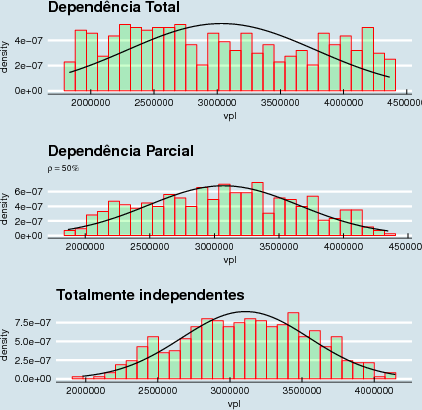
\includegraphics[width=0.7\linewidth]{images/histogramasuniforme-1} 

}

\caption{Gráficos -- Distribuição \emph{a priori}: uniforme}\label{fig:histogramasuniforme}
\end{figure}

\subsubsection{Simulação de Monte Carlo com distribuição
beta}\label{simulacao-de-monte-carlo-com-distribuicao-beta}

Da mesma maneira explicada na seção anterior, realizamos 500 simulações
com a distribuição beta. Neste caso, adotamos como parâmetros da
distribuição beta os fatores \(\alpha\) e \(\beta\) iguais a 2 e 2,
respectivamente.

\paragraph{A distribuição beta}\label{a-distribuicao-beta}

A distribuição beta está definida no intervalo (0,1) e pode assumir
diferentes formas dentro deste intervalo, motivo pelo qual a
distribuição beta é um modelo conveniente para prever o comportamento
aleatório de porcentagens e proporções. Dependendo dos fatores de forma
\(\alpha\) e \(\beta\) adotados. Quando os valor de \(\alpha\) e
\(\beta\) são simultaneamente iguais a 1, a distribuição beta toma a
forma da distribuição uniforme no intervalo (0,1). Mas a distribuição
beta pode tomar uma variedade de formas para outros valores de
\(\alpha\) e \(\beta\), alguns dos quais podem ser vistos abaixo:

\begin{figure}[H]

{\centering 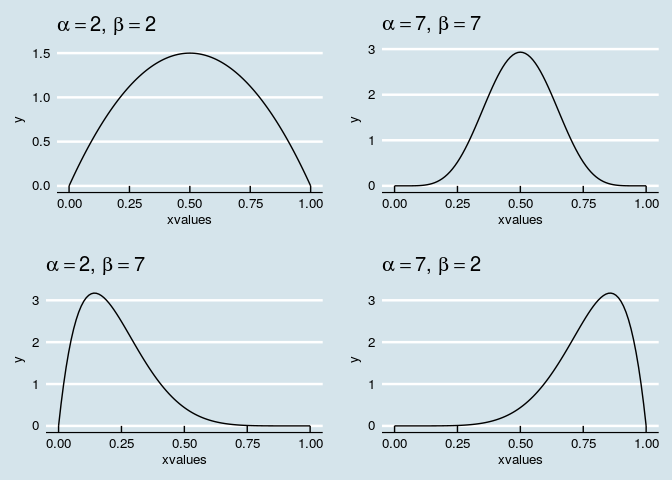
\includegraphics[width=0.7\linewidth]{images/variasbeta-1} 

}

\caption{Gráficos Distribuição beta -- vários fatores de forma}\label{fig:variasbeta}
\end{figure}

É normalmente utilizada na inferência Bayesiana como distribuição a
priori, onde os parâmetros \(\alpha\) e \(\beta\) são inicialmente
estimados e posteriormente atualizados de acordo com os resultados de
pesquisas.

Na inferência Bayesiana, os parâmetros podem ser inicialmente estimados
de acordo com o conhecimento empírico prévio do especialista. Como
exemplo, imagine que um orçamentista deseje testar se o Custo Unitário
Básico (CUB) divulgado pelo SINDUSCON/SC para um determinado padrão de
construção é uma boa estimativa para o custo médio das obras daquele
padrão no seu município. O orçamentista experiente estima que os custos
de construção das obras daquele padrão se situem entre 90\% e 110\% do
CUB e, inicialmente, pensa que o CUB é sim um bom estimador dos custos
de construção para o seu município, por isto ele prevê que 50\% das
obras daquele padrão tenham custo de construção menor ou igual ao CUB,
enquanto as outras 50\% a superem. Ainda, o especialista prevê que, para
aquele padrão, apenas 10\% das obras tenham custo abaixo de 95\% do CUB
(ou seja, se encontrem no primeiro quartil).

Isto equivale a dizer que o especialista pode utilizar uma distribuição
beta como a mostrada abaixo como uma distribuição a priori do custo das
obras no seu município:

\begin{Shaded}
\begin{Highlighting}[]
\KeywordTok{beta_area}\NormalTok{(}\DecValTok{0}\NormalTok{, }\FloatTok{0.25}\NormalTok{, }\KeywordTok{c}\NormalTok{(}\FloatTok{3.09}\NormalTok{, }\FloatTok{3.09}\NormalTok{))}
\end{Highlighting}
\end{Shaded}

\begin{figure}[H]

{\centering \includegraphics[width=0.7\linewidth]{images/beta_area-1} 

}

\caption{Distribuição Beta: obtenção dos fatores de forma à partir das proporções imaginadas \emph{a priori}}\label{fig:beta_area}
\end{figure}

Posteriormente, o orçamentista realiza uma pesquisa com 20 obras de
construtoras locais e verifica que apenas 7 tiveram custo inferior ao
CUB. Com estes dados, o especialista deve atualizar a sua distribuição
de probabilidade a priori, obtendo uma distribuição a posteriori que se
compara com a distribuição a priori da seguinte maneira:

\begin{Shaded}
\begin{Highlighting}[]
\NormalTok{data <-}\StringTok{ }\KeywordTok{c}\NormalTok{(}\DecValTok{13}\NormalTok{, }\DecValTok{7}\NormalTok{)}
\NormalTok{post_par <-}\StringTok{ }\NormalTok{prior_par }\OperatorTok{+}\StringTok{ }\NormalTok{data}
\KeywordTok{beta_prior_post}\NormalTok{(prior_par, post_par)}
\end{Highlighting}
\end{Shaded}

\begin{figure}[H]

{\centering \includegraphics[width=0.7\linewidth]{images/betapriorpost-1} 

}

\caption{Distribuição Beta \emph{a posteriori} -- atualização da forma à partir de pesquisas.}\label{fig:betapriorpost}
\end{figure}

Este processo pode ser repetido continuamente, com a distribuição a
posteriori tornando-se a nova distribuição a priori e realizando-se nova
pesquisa.

\paragraph{Dependência Total}\label{dependencia-total}

A probabilidade que o VPL seja inferior a 85\% da média pode ser
calculado através do número de simulações com valor abaixo deste valor,
dividido pelo número de simulações:

\begin{Shaded}
\begin{Highlighting}[]
\KeywordTok{sum}\NormalTok{(vpl_beta2_}\DecValTok{100}\OperatorTok{$}\NormalTok{vpl }\OperatorTok{<}\StringTok{ }\FloatTok{0.85}\OperatorTok{*}\KeywordTok{mean}\NormalTok{(vpl_beta2_}\DecValTok{100}\OperatorTok{$}\NormalTok{vpl))}\OperatorTok{/}\NormalTok{Nsim}
\end{Highlighting}
\end{Shaded}

\begin{verbatim}
## [1] 0.222
\end{verbatim}

Ou teoricamente, através da função densidade de probabilidade normal,
com os parâmetros iguais aos da simulação, a saber, média de
\textbf{3.065.854,04} e desvio padrão \textbf{556.617,97}:

\begin{Shaded}
\begin{Highlighting}[]
\KeywordTok{pnorm}\NormalTok{(}\FloatTok{0.85}\OperatorTok{*}\KeywordTok{mean}\NormalTok{(vpl_beta2_}\DecValTok{100}\OperatorTok{$}\NormalTok{vpl), }\DataTypeTok{mean =} \KeywordTok{mean}\NormalTok{(vpl_beta2_}\DecValTok{100}\OperatorTok{$}\NormalTok{vpl), }\DataTypeTok{sd =} \KeywordTok{sd}\NormalTok{(vpl_beta2_}\DecValTok{100}\OperatorTok{$}\NormalTok{vpl))}
\end{Highlighting}
\end{Shaded}

\begin{verbatim}
## [1] 0.2043452
\end{verbatim}

\paragraph{Dependência Parcial}\label{dependencia-parcial}

A probabilidade que o VPL seja inferior a 85\% da média pode ser
calculado através do número de simulações com valor abaixo deste valor,
dividido pelo número de simulações:

\begin{Shaded}
\begin{Highlighting}[]
\KeywordTok{sum}\NormalTok{(vpl_beta2_}\DecValTok{50}\OperatorTok{$}\NormalTok{vpl }\OperatorTok{<}\StringTok{ }\FloatTok{0.85}\OperatorTok{*}\KeywordTok{mean}\NormalTok{(vpl_beta2_}\DecValTok{50}\OperatorTok{$}\NormalTok{vpl))}\OperatorTok{/}\NormalTok{Nsim}
\end{Highlighting}
\end{Shaded}

\begin{verbatim}
## [1] 0.174
\end{verbatim}

Ou teoricamente, através da função densidade de probabilidade normal,
com os parâmetros iguais aos da simulação, a saber, média de
\textbf{3.100.073,94} e desvio padrão \textbf{480.802,12}:

\begin{Shaded}
\begin{Highlighting}[]
\KeywordTok{pnorm}\NormalTok{(}\FloatTok{0.85}\OperatorTok{*}\KeywordTok{mean}\NormalTok{(vpl_beta2_}\DecValTok{50}\OperatorTok{$}\NormalTok{vpl), }\DataTypeTok{mean =} \KeywordTok{mean}\NormalTok{(vpl_beta2_}\DecValTok{50}\OperatorTok{$}\NormalTok{vpl), }\DataTypeTok{sd =} \KeywordTok{sd}\NormalTok{(vpl_beta2_}\DecValTok{50}\OperatorTok{$}\NormalTok{vpl))}
\end{Highlighting}
\end{Shaded}

\begin{verbatim}
## [1] 0.1667328
\end{verbatim}

\paragraph{Independência Total}\label{independencia-total}

A probabilidade que o VPL seja inferior a 85\% da média pode ser
calculado através do número de simulações com valor abaixo deste valor,
dividido pelo número de simulações:

\begin{Shaded}
\begin{Highlighting}[]
\KeywordTok{sum}\NormalTok{(vpl_beta2}\OperatorTok{$}\NormalTok{vpl }\OperatorTok{<}\StringTok{ }\FloatTok{0.85}\OperatorTok{*}\KeywordTok{mean}\NormalTok{(vpl_beta2}\OperatorTok{$}\NormalTok{vpl))}\OperatorTok{/}\NormalTok{Nsim}
\end{Highlighting}
\end{Shaded}

\begin{verbatim}
## [1] 0.092
\end{verbatim}

Ou teoricamente, através da função densidade de probabilidade normal,
com os parâmetros iguais aos da simulação, a saber, média de
\textbf{3.073.671,40} e desvio padrão \textbf{339.347,82}:

\begin{Shaded}
\begin{Highlighting}[]
\KeywordTok{pnorm}\NormalTok{(}\FloatTok{0.85}\OperatorTok{*}\KeywordTok{mean}\NormalTok{(vpl_beta2}\OperatorTok{$}\NormalTok{vpl), }\DataTypeTok{mean =} \KeywordTok{mean}\NormalTok{(vpl_beta2}\OperatorTok{$}\NormalTok{vpl), }\DataTypeTok{sd =} \KeywordTok{sd}\NormalTok{(vpl_beta2}\OperatorTok{$}\NormalTok{vpl))}
\end{Highlighting}
\end{Shaded}

\begin{verbatim}
## [1] 0.08713072
\end{verbatim}

\paragraph{Gráficos}\label{graficos-1}

\begin{figure}[H]

{\centering 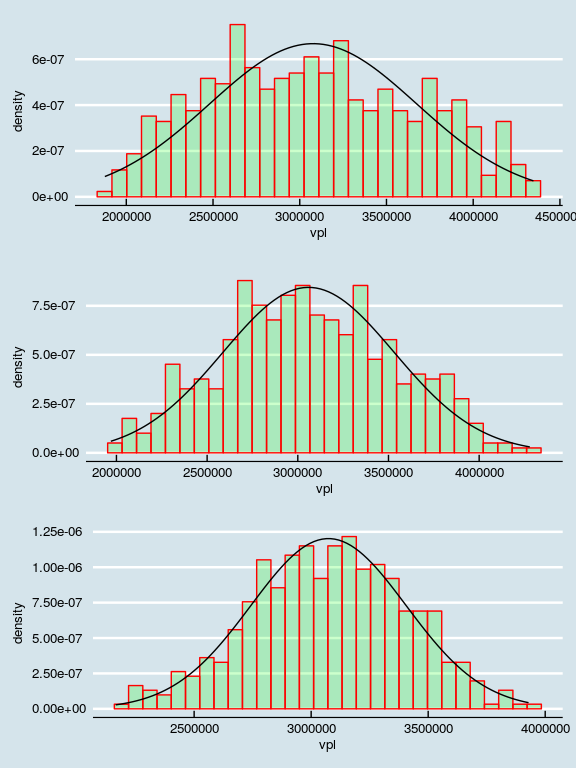
\includegraphics[width=0.7\linewidth]{images/histogramasbeta-1} 

}

\caption{Gráficos -- Distribuição \emph{a priori}: Beta 2}\label{fig:histogramasbeta}
\end{figure}

\paragraph{Mudança de parâmetros da distribuição
beta}\label{mudanca-de-parametros-da-distribuicao-beta}

No entanto, não há motivos para supor que as variáveis aleatórias
assumam uma distribuição beta com os parâmetros descritos na seção
anterior.

Para efeito de comparação, abaixo efetuamos outra simulação, desta vez
com parâmetros \(\alpha\) e \(\beta\) iguais a 7 e 7, respectivamente,
com variáveis aleatórias completamente independentes.

A probabilidade que o VPL seja inferior a 85\% da média pode ser
calculado através do número de simulações com valor abaixo deste valor,
dividido pelo número de simulações:

\begin{Shaded}
\begin{Highlighting}[]
\KeywordTok{mean}\NormalTok{(vpl_beta7}\OperatorTok{$}\NormalTok{vpl }\OperatorTok{<}\StringTok{ }\FloatTok{0.85}\OperatorTok{*}\KeywordTok{mean}\NormalTok{(vpl_beta7}\OperatorTok{$}\NormalTok{vpl))}
\end{Highlighting}
\end{Shaded}

\begin{verbatim}
## [1] 0.002
\end{verbatim}

Ou teoricamente, através da função densidade de probabilidade normal,
com os parâmetros iguais aos da simulação, a saber, média de
3.090.242,33 e desvio padrão 199.387,61:

\begin{Shaded}
\begin{Highlighting}[]
\KeywordTok{pnorm}\NormalTok{(}\FloatTok{0.85}\OperatorTok{*}\KeywordTok{mean}\NormalTok{(vpl_beta7}\OperatorTok{$}\NormalTok{vpl), }\DataTypeTok{mean =} \KeywordTok{mean}\NormalTok{(vpl_beta7}\OperatorTok{$}\NormalTok{vpl), }\DataTypeTok{sd =} \KeywordTok{sd}\NormalTok{(vpl_beta7}\OperatorTok{$}\NormalTok{vpl))}
\end{Highlighting}
\end{Shaded}

\begin{verbatim}
## [1] 0.01004132
\end{verbatim}

\begin{figure}[H]

{\centering 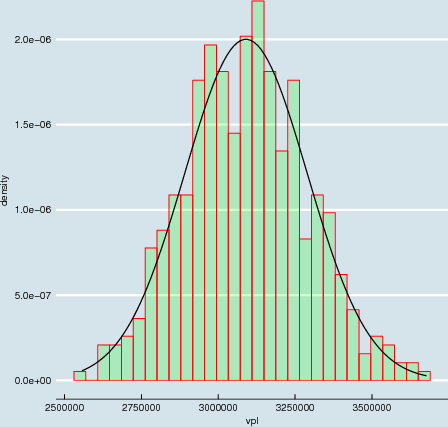
\includegraphics[width=0.7\linewidth]{images/histbeta7-1} 

}

\caption{Gráfico -- Distribuição \emph{a priori}: Beta 7 -- Independência Total}\label{fig:histbeta7}
\end{figure}

\subsection{Estatísticas descritivas}\label{estatisticas-descritivas}

\rowcolors{2}{gray!6}{white}

\begin{table}

\caption{\label{tab:estat_descr}Estatísticas descritivas das diferentes simulações}
\centering
\begin{tabular}[t]{lrrrrrr}
\hiderowcolors
\toprule
  & Min. & 1st Qu. & Median & Mean & 3rd Qu. & Max.\\
\midrule
\showrowcolors
s\_unif\_100 & 1.830.675 & 2.397.169 & 2.977.241 & 3.033.769 & 3.704.561 & 4.363.364\\
s\_unif\_50 & 1.866.410 & 2.614.612 & 3.091.766 & 3.070.837 & 3.536.131 & 4.345.420\\
s\_unif & 1.977.606 & 2.777.265 & 3.113.936 & 3.107.640 & 3.441.087 & 4.146.205\\
s\_beta2\_100 & 1.910.691 & 2.658.857 & 3.061.174 & 3.065.854 & 3.519.846 & 4.327.316\\
s\_beta2\_50 & 1.907.261 & 2.749.625 & 3.063.516 & 3.100.074 & 3.452.953 & 4.306.794\\
\addlinespace
s\_beta2 & 2.219.450 & 2.833.522 & 3.048.477 & 3.073.671 & 3.316.966 & 4.067.581\\
s\_beta7 & 2.557.123 & 2.952.993 & 3.091.660 & 3.090.242 & 3.227.009 & 3.677.510\\
\bottomrule
\end{tabular}
\end{table}

\rowcolors{2}{white}{white}

\rowcolors{2}{gray!6}{white}

\begin{table}[H]

\caption{\label{tab:resumo}Resumo das médias e desvios}
\centering
\begin{tabular}[t]{llrr}
\hiderowcolors
\toprule
Distribuição & Dependência & Média & Desvio\_Padrão\\
\midrule
\showrowcolors
Uniforme & Total & 3.033.769 & 746.342,7\\
Uniforme & Parcial (50\%) & 3.070.837 & 586.336,8\\
Uniforme & Independente & 3.107.640 & 443.892,3\\
Beta & Total & 3.065.854 & 556.618,0\\
Beta & Parcial (50\%) & 3.100.074 & 480.802,1\\
\addlinespace
Beta & Independente & 3.073.671 & 339.347,8\\
Beta & Independente & 3.090.242 & 199.387,6\\
\bottomrule
\end{tabular}
\end{table}

\rowcolors{2}{white}{white}

\section{Conclusão}\label{conclusao}

Como notamos nas últimas seções, o valor médio das simulações pouco se
altera com a mudança das distribuições adotadas. No entanto, o
desvio-padrão das simulações é alterado drasticamente com a mudança da
distribuição ou dos parâmetros adotados para elas.

Pesquisas devem ser feitas no sentido de estimar parâmetros mais
precisos de distribuição das variáveis envolvidas.

\section*{Referências}\label{referencias}
\addcontentsline{toc}{section}{Referências}

\hypertarget{refs}{}
\hypertarget{ref-LearnBayes}{}
ALBERT, J. \textbf{LearnBayes: Functions for learning bayesian
inference}. 2014.

\hypertarget{ref-appraiseR}{}
DROUBI, L. \textbf{AppraiseR: Tools for real estate appraisal}. 2018.

\hypertarget{ref-Copulas}{}
GOLDFELD, K. Copulas and correlated data generation: Getting beyond the
normal distribution. Disponível em:
\textless{}\url{https://www.rdatagen.net/post/correlated-data-copula/}\textgreater{}.
Acesso em: 8/2/2018.

\hypertarget{ref-hoccheim2}{}
HOCCHEIM, N. \textbf{Avaliação de terrenos e glebas pelo método
involutivo}. Florianópolis: IBAPE - SC, 2017.

\hypertarget{ref-econometrics}{}
SMART, F. Easily generate correlated variables from any distribution.
Disponível em:
\textless{}\url{https://www.rdatagen.net/post/correlated-data-copula/}\textgreater{}.
Acesso em: 8/2/2018.

\hypertarget{ref-MASS}{}
VENABLES, W. N.; RIPLEY, B. D. \textbf{Modern applied statistics with
s}. Fourth ed. New York: Springer, 2002.


\end{document}
